\documentclass[slidestop,compress,mathserif]{beamer}
\mode<presentation>
\beamertemplatenavigationsymbolsempty
\addtobeamertemplate{navigation symbols}{}{%
	\usebeamerfont{footline}%
	\usebeamercolor[fg]{footline}%
	\hspace{5em}%
	\textbf{\insertframenumber/\inserttotalframenumber}
}
\usepackage[outputdir=build]{minted}
\usepackage{latexsym}
\usepackage{menukeys}
\usepackage{bytefield}
\usepackage{textcomp}

\usepackage{tikz}
\usetikzlibrary{shapes,arrows}

%\usepackage[bars]{beamerthemetree} % Beamer主题样式v 2.2
\usetheme{Antibes} % Beamer主题样式v 3.0
\usecolortheme{lily} % Beamer颜色主题样式

\AtBeginSubsection[]{
	\begin{frame}
	\vfill
	\centering
	\begin{beamercolorbox}[sep=8pt,center,shadow=true,rounded=true]{title}
		\insertsectionhead\newline\newline\usebeamerfont{title}\insertsubsectionhead\par%
	\end{beamercolorbox}
	\vfill
	\end{frame}
}

\title{VE280 Recitation Class Notes}
\author{YAO Yue}
\institute{VE280 SU17 TA Group}
\begin{document}
	\begin{frame} % Cover slide
	\titlepage
	
	\tiny{Source code available at https://github.com/tripack45/VE280-Notes}
	\end{frame}
	
	\begin{frame}[allowframebreaks]
		\frametitle{Table Of Contents}
		\tableofcontents
	\end{frame}

		\section{RC Week 2}
		\subsection{OK, VE280. What is this course?}
		\begin{frame}
	\frametitle{How to write good code ${}^\text{and linked lists}$}	
	\begin{block}{Writing Quality Code}
		\begin{description}[Motivation]
					\item[Taste] What kind of code are considered "good"?
					\item[Motivation] What benefit would such code give us?
					\item[Techique] What is the recipe for such code?
					\item[Tools] What language features does C++ provide for achieving this goal? How to use them?
				\end{description}
				\small{Good (Bad?) News: Exams will (mostly) test for the last point.}
			\end{block}
			\begin{block}{Elementary Data Structure}
				Singly linked lists, Doubly linked lists, Circular Arrays ... \
			\end{block}
		\end{frame}
		\begin{frame}{OK, "Quality Code"?}
			It's very hard to give a definition.
			\begin{columns}
				\column[]{.5\textwidth}
				
				\begin{block}{Good Code}
					\begin{itemize}
						\item Good variable names
						\item Consistent indentation
						\item Well tested, documented
						\item D-R-Y, Don't repeat yourself
						\item High Coherence / Low coupling
						\item Open for extension, but closed for modification
					\end{itemize}
				\end{block}
				\column[]{.5\textwidth}
				\begin{block}{Bad Code}
					\begin{itemize}
						\item Bad Style
						\item 200+ lines in a one function
						\item Functions of 20+ Args
						\item Magic numbers everywhere
						\item Seriously you know bad code when you see one (write one).
					\end{itemize}
				\end{block}
			\end{columns}
			Many of them are related to \emph{Abstraction}.
		\end{frame}
	
\begin{frame}[fragile]{Head First \textit{Abstraction}}
	\framesubtitle{No abstraction}
	\begin{block}{The Requirement}
		\textit{CubedEnix (CE)} is trying to develop a third person shooting game called \textit{World of Armored Blizzard} (WOAB). In this game, AI will control a tank that can fire upon the player. A programmer \textit{Archer} is asked to implement this feature. 
	\end{block}
	\begin{block}{The Solution}
		Archer propose to have a global variable \texttt{TANK} of class \texttt{Tank} to represent the tank. Archer than writes the following code.
\begin{minted}{c++}
...
Player target = TANK.aim(); TANK.fire(target);
...
\end{minted}
		Archer feels happy, so does his boss.
	\end{block}
\end{frame}

\begin{frame}[fragile]{Head First \textit{Abstraction}}
	\framesubtitle{No abstraction}
	\begin{block}{Change of Requirement}
		Players are complaining that the game is too easy. WOAB dev team decided to add 2 more AI controlled tanks. Again Archer is asked to implement it.
	\end{block}
	\begin{block}{The Solution}
		Archer decided to use 3 global variables \texttt{TANK0, TANK1, TANK2} of class \texttt{Tank}. He copies the original code into 3 different places and modify each of them.
		\begin{minted}{c++}
... Player target = TANK0.aim(); TANK0.fire(target);
... Player target = TANK1.aim(); TANK1.fire(target);
... Player target = TANK2.aim(); TANK2.fire(target);
		\end{minted}
		Archer feels happy, so does his boss.
	\end{block}
\end{frame}

\begin{frame}[fragile]{Head First \textit{Abstraction}}
	\framesubtitle{No abstraction}
	\begin{block}{Change of Requirement}
		Within the next 2 months they increased number of tanks to 10. 1 year later, they (finally!) decided to play a sound effect when a tank fires. 
	\end{block}
	\begin{block}{The Twist}
		Archer now has 10 copies! He needs to add a function call \texttt{playSound()} to each copy. Unfortunately he missed one location.  Archer also doesn't test his code.  Now Buggy code is released.
		
		Players are unhappy. His boss is unhappy. Archer is fired. Archer is unhappy. Lancer takes his job.
	\end{block}
\end{frame}

\begin{frame}[fragile]{Head First \textit{Abstraction}}
	\framesubtitle{With Procedual Abstraction}
	\begin{block}{The Solution}
		Lancer decided to write a function that takes a \texttt{Tank} object as an argument.
		\begin{minted}{c++}
// Argument: A non-null pointer to a Tank object.
// Effect  : Fires such tank on the current player.
void tankFire(Tank* t) {
    playSound();
    Player target = t->takeAim(); 
    t->fire(target);
}
		\end{minted}
		With this new design Lancer can easily change the number of \texttt{TANK}s in the game, or modify the how tanks fire by simply changing this single function.
	\end{block}
\end{frame}

\begin{frame}[fragile]{Head First \textit{Abstraction}}
\framesubtitle{With just procedual abstraction}
\begin{block}{Change of Requirement}
	\small{You know what? Those player just can't be satisfied. WOAB dev team now decides to involve not just tanks but also battle ships and planes (and witches and dragons ...). Lancer is asked to implement "fire" feature for all of them.}
\end{block}
\begin{block}{The Twist}
	\small{Lancer is now in a tough situation. Clearly Tanks, Ships, Planes... are different things. Their attack would have different effects. There won't be a single function that works for all of them.
	
	Since Lancer didn't take VE280 seriously when he is in JI, Lancer falls back to copying the code for each "character" once. After 2 months, the code is no longer maintainable, and thus he is fired. Saber takes his job.}
\end{block}
\end{frame}

\begin{frame}[fragile]{Head First \textit{Abstraction}}
\framesubtitle{With Data Abstraction}
\begin{block}{The Solution}
The key is to see the elephant in the room. What's the common characteristic of tanks, ships, dragons and witches? They all attack our player!
\begin{minted}{c++}
class IAttackPlayer {
    virtual void fire(Player p) = 0;
    virtual Player takeAim() = 0;
}
class Tank : public IAttackPlayer;
class Ship : public IAttackPlayer;
....
\end{minted}
\end{block}
\end{frame}

\begin{frame}[fragile]{Head First \textit{Abstraction}}
\framesubtitle{With Data Abstraction}
\begin{block}{The Solution}
	Then we can modify the function:
	\begin{minted}{c++}
// Argument: a object implements IAttackPlayer.
// Effect  : Fires such tank on the current player.
void NpcFire(IAttackPlayer* t) {
    playSound();
    Player target = t->takeAim(); 
    t->fire(target);
}
	\end{minted}
	In the above design Saber abstracted out what the thing "physically" is. She defines things by defining what it can do.
\end{block}
\end{frame}

\begin{frame}{A few more words}
\begin{block}{It's okay if You don't fully understand above story}
	That's gives you a good reason to learn it well.
\end{block}
\begin{block}{Can you talk something about projects?}
	Well, projects are mostly very direct. Be careful in the process and they should be pretty easy. Reserve around 5 days for them.
	
	Remember it's easy to simply finish them. But to finish them elegantly trust me when I say it's hard. 
	
	Yes, it's hard. But the outcome worth every minute spent.
\end{block}
\end{frame}

\subsection{Your Linux Operating System}
\begin{frame}{Linux as a operating system \textit{kernel}}
\begin{block}{Operating systems as a resource manager}
	Operating systems manage your hardware. These include computation resource (CPU, GPU), storage (Hard drive), communication resource (network)...
\end{block}
\begin{block}{The core of OS, a.k.a. \textit{kernel}}
	At the very heart of the OS there lies the kernel. This piece of software talks directly to the hardware. It provides a unified way of accessing your storage devices (Filesystems), graphic devices, network...
\end{block}
\begin{block}{``Linux" is first the name of the kernel}
	This implies you can actually change your desktop environment: fancier? go with Unity/KDE/Gnome. Light weight \& fast? go with LXDE or XFCE. 
\end{block}
\end{frame}

\begin{frame}{Flavors of Linux: \textit{Distributions}}
\framesubtitle{Common Choices}
\begin{small}
	This flexibility of choice allows to tailor the system towards our own need. Some commonly accepted configurations become "Distributions".
\end{small} 
\begin{block}{Ubuntu Series}
	Maintained by Canonical, it's actually a series of distributions with different choice of desktop environment. Ubuntu / \textit{Unity}. Kubuntu / \textit{KDE}. Lubuntu / \textit{LXDE}. Xubuntu / \textit{XFCE}. Use \textit{apt}.
\end{block}
\begin{block}{Debian}
	Once the most widely use distribution, the father of Ubuntu [that's right :=)]. Package management system is \textit{apt}
\end{block}
\begin{block}{Fedora and RedHat Linux Enterprise}
	Maintained by Red Hat. Fedora is new and cutting edge. RedHat now focus on enterprises. Package Management is \textit{yum/dnf}.
\end{block}
\end{frame}

\begin{frame}{Flavors of Linux: \textit{Distributions}}
\framesubtitle{Uncommon choices}
\begin{block}{Open SUSE}
	Maintained by german company SUSE. Focus on stability. 
\end{block}
\begin{block}{Arch Linux / Manjaro}
	ROLLING UPDATE! Absolutely cutting edge. Great community and wiki. User is assumed to be experienced. Installation of Arch Linux is done on command line while Manjaro makes easier. Package management system is \textit{pacman}.
\end{block}
\begin{block}{Linux From Scratch (LFS) / Gentoo}
	Try LFS if you are absolutely interested in figuring out how everything works. Think LFS is crazy enough? Well Gentoo compiles every piece of software you use FROM THE SOURCE! 
\end{block}
\end{frame}

\begin{frame}{Bash on Windows Subsystem for Linux}
\begin{block}{Think big, with abstraction}
	For Linux programs, technically, you don't need an "real" linux kernel to run them. As long as you have some thing that looks like a real one (one that follows the same abstraction). 
\end{block}
\begin{block}{Windows Subsystem for Linux}
	This year Microsoft actually release one. Installation guide is available \href{https://msdn.microsoft.com/zh-cn/commandline/wsl/install\_guide}{here(click me)}.
	
	This solution is easy to use, clean. It saves you time copying files back and forth from the virtual machine. You can simply develop in Windows using your favorite tool (IDE and test it easily under ``Linux''. It's a good solution for the purpose of this course.
\end{block}
\end{frame}

\begin{frame}{Virtual Machines vs. Containers}
\begin{block}{Virtual Machines}
	A virtual machine (VM) is an emulation of a computer system. Virtual machines are based on computer architectures and provide functionality of a physical computer. The CPUs, memory, kernel, file systems and devices are all virtualized and need translation, which makes it slower than a physical computer.
\end{block}
\begin{block}{Containers}
	A container shares the CPUs, memory, kernel, file systems and devices with the host machine, which makes it almost as fast as the host machine when executing machine code (no virtualization means no translation of machine code). Everything in a container is something mapped from the host system. \structure{Docker} is a lighweighted, standalone and secure container daemon which is very popular nowadays.
\end{block}
\end{frame}

\begin{frame}[fragile]{Aspects of Linux: Users}
\vspace{-0.12in}
\begin{description}[Permission]
	\small
	\item[MultiUser] Multiple person can operate the system at once.
	\item[Group] Each User belongs to one or more groups
	\item[Home Dir] Each user has his/her own directory under \texttt{/home}
	\item[$\sim$/] Shorthand for home directory. This one is user specific.
	\item[Premission] Owner/Group/Other Read/Write/Execute Flags
	\item[root] A special super user \texttt{root} overrides all security 
	\item[su] Command that starts a temporary shell as \texttt{root}
	\item[sudo] A command that temporarily grant superuser privilege to current user. Namely, ``execute the following command as `root`". 
\end{description}
\small{The Miranda warning of \texttt{sudo}:}
\begin{minted}[fontsize=\footnotesize]{text}
We trust you have received the usual lecture from the local 
System Administrator. It usually boils down to these three things:
    #1) Respect the privacy of others.
    #2) Think before you type.
    #3) With great power comes great responsibility.
root's password:
\end{minted}
\end{frame}

\begin{frame}{Aspects of Linux: Filesystem}
\begin{block}{Filesystem is an abstraction of storage}
	That's right, abstraction again. Filesystem hides the physical storage schema of your files. Instead it should reflect how your files are logically organized.
\end{block}
\begin{block}{Linux Filesystem}
	In Linux files are organized in a tree-like structure.
	\begin{figure}
		\vspace{-0.2in}
		\centering
		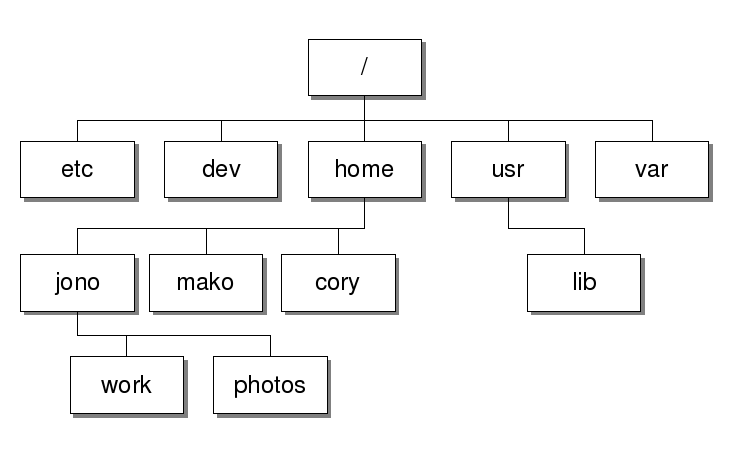
\includegraphics[scale=0.5]{fig/rc2_linuxfs}
	\end{figure}
\end{block}
\end{frame}

\begin{frame}{Aspects of Linux: Filesystem}
\framesubtitle{Caveats for the names}

\begin{block}{A word from Ken Thompson}
\begin{quote}
	Ken Thompson was once asked what he would do differently if he were redesigning the UNIX system. His reply: "I'd spell creat with an e."
\end{quote}
\end{block}

\vspace{-0.15in}
\begin{columns}
	\column{.5\textwidth}
	\begin{description}[/boot]
	\item[/bin] \textbf{Bin}aries
	\item[/dev] \textbf{Dev}ices
	\item[/boot] \textbf{Boot}strap
	\item[/sbin] \textbf{S}ecure \textbf{bin}aries
	\end{description}
	\column{.5\textwidth}
	\begin{description}[/home]
	\item[/mnt] \textbf{M}ou\textbf{nt}ed filesystem
	\item[/etc] Configuration files
	\item[/usr] \textbf{U}nix \textbf{s}ystem \textbf{r}esources
	\item[/home] Places for the user's files
	\end{description}
\end{columns}

\vspace{0.1in} \tiny{More at https://wiki.debian.org/FilesystemHierarchyStandar}
\end{frame}

\begin{frame}{Aspects of Linux: Shell}

\begin{block}{CLI and Shell}
\textbf{C}ommand \textbf{L}ine \textbf{I}nterface is fast, consumes minimum resources and effective. \textbf{G}raphical \textbf{U}ser \textbf{I}nterface comes with a much larger cost. 

Management tasks are generally easier on CLI (think about coding!).

The program that interprets user commands and provides feedbacks is called a \textit{Shell}. When you login to the computer, the shell runs automatically. You interact with the computer through the shell. 
\end{block}

\begin{block}{Differenct choices of shell}
	The ``standard" one on most linux is \texttt{bash}, as in ``\textbf{B}ourne's \textbf{A}gain \textbf{Sh}ell". But choices like \texttt{zsh}, \texttt{fish}, \texttt{csh} are much more easier to use (cooler). Checkout the ``oh-my-zsh" project on GitHub if you are interested.
\end{block}
\end{frame}

\begin{frame}{Aspects of Linux: Shell}
\framesubtitle{The working directory}
	How does \texttt{fopen("test.txt")} work? I mean, how does the computer know where to find \texttt{text.txt}? 
	
	Each program is associated with a special directory called ``working directory". Normally this is the directory where you execute the program. (Not where the program is!). 

\begin{block}{Related commands}
	\small
	\begin{description}[pwd]
		\item[pwd] \textbf{P}rint \textbf{w}orking \textbf{d}irectory
		\item[cd] \textbf{C}hange \textbf{d}irectory. Each directory has 2 very special ``sub-directory". ``\textbf{./}" and ``\textbf{../}". They are logically sub-directory. Meaning you can do \texttt{cd /home/john/./} and \texttt{cd /home/john/../}, but the in fact, the first command takes you to \texttt{/home/john/} and the second one takes you to \texttt{/home/}. 
		
		``\texttt{cd ./}" keeps where you are and ``\texttt{cd ../}"" takes you 1 level up.
	\end{description}
	

\end{block}
\end{frame}

\begin{frame}[fragile]{Aspects of Linux: Shell}
\framesubtitle{Executing programs}
The general syntax is 
\begin{minted}{bash}
executable_file arg1 arg2 arg3 ...
\end{minted}
Conventions are:\\
1) arguments begin with \texttt{-} are called "switches" or "options" \\
2) one dash (one \texttt{-}) are called short switches, e.g. \texttt{-l}, \texttt{-a}\\
3) short switch always uses single letter to specify. Case / lower letters can have very different meanings! Be very careful.
3) multiple short switches can often be specified at once. e.g. \texttt{ls -al}\\
4) two dashes (one \texttt{-}) are called long switches, e.g. \texttt{--all}, \texttt{--mode=linear}. Usually long switches use whole words other than acronyms.\\
5) \textbf{THERE ARE OUTLIERS!}. Unfortunately \texttt{gcc} and \texttt{g++} are two of these naughty boys. 
\end{frame}

\begin{frame}{Aspects of Linux: Shell}
\framesubtitle{Useful commands}
	\begin{description}[mkdir]
		\item[ls] \textbf{L}i\textbf{s}t files \& folders under a directory. This command takes zero or more arguments. If the argument is a directory, list that dir. If the argument is a file, show information of that specific file. If no arguments are given, list working directory.
		\begin{description}[-a]
			\small
			\item[-a] List hidden files as well. Leading dot means ``hidden".
			\item[-l] Use \textbf{l}ong format. Each line for a single file. 
		\end{description}
		\item[mkdir] \textbf{M}a\textbf{k}e \textbf{dir}ectory, self-explanatory.
		\item[rm] \textbf{R}e\textbf{m}ove files / directory. It is \textbf{extremely dangerous} to run \texttt{rm} with administrative privilege! See the bumblebee accident. \url{https://github.com/MrMEEE/bumblebee-Old-and-abbandoned/issues/123}
		\begin{description}[-a]
			\small
			\item[-r] Deletes files/folders recursively. Folders requires this option.
			\item[-f] Force remove. Ignores warnings.  
		\end{description}
		\item[rmdir] \textbf{R}e\textbf{m}ove \textbf{dir}ectory, only \textbf{empty} ones can be removed.
	\end{description}

\end{frame}


\begin{frame}{Aspects of Linux: Shell}
\framesubtitle{Useful commands, Cont'd}
\begin{description}[mkdir]
	\item[touch] Designed to change the time stamp of file. Commonly used to create an empty file.
	\item[cp] \textbf{C}o\textbf{p}y files/folder. Takes 2 arguments \texttt{source} and \texttt{dest}. Be very careful if both \texttt{source} and \texttt{dest} are both existing folders. Try it yourself!
	\begin{description}[-]
		\small
		\item[-r] Copy files/folders recursively. Folders requires this option.  
	\end{description}
	\item[mv] \textbf{M}o\textbf{v}e files / directory. Takes 2 arguments \texttt{source} and \texttt{dest}. If \texttt{source} and \texttt{dest} is the same location, this command essentially does a rename. Pay attention to the situation where both arguments are already existed.
	\item[cat] Con\textbf{cat}enate files. Takes multiple arguments and print their content one by one to \texttt{stdout}. When there is just one argument, it essentially displays the content.
\end{description}
\end{frame}


\begin{frame}{Aspects of Linux: Shell}
\framesubtitle{Long Format of File Information}
	\begin{figure}
		\vspace{-0.2in}
		\centering
		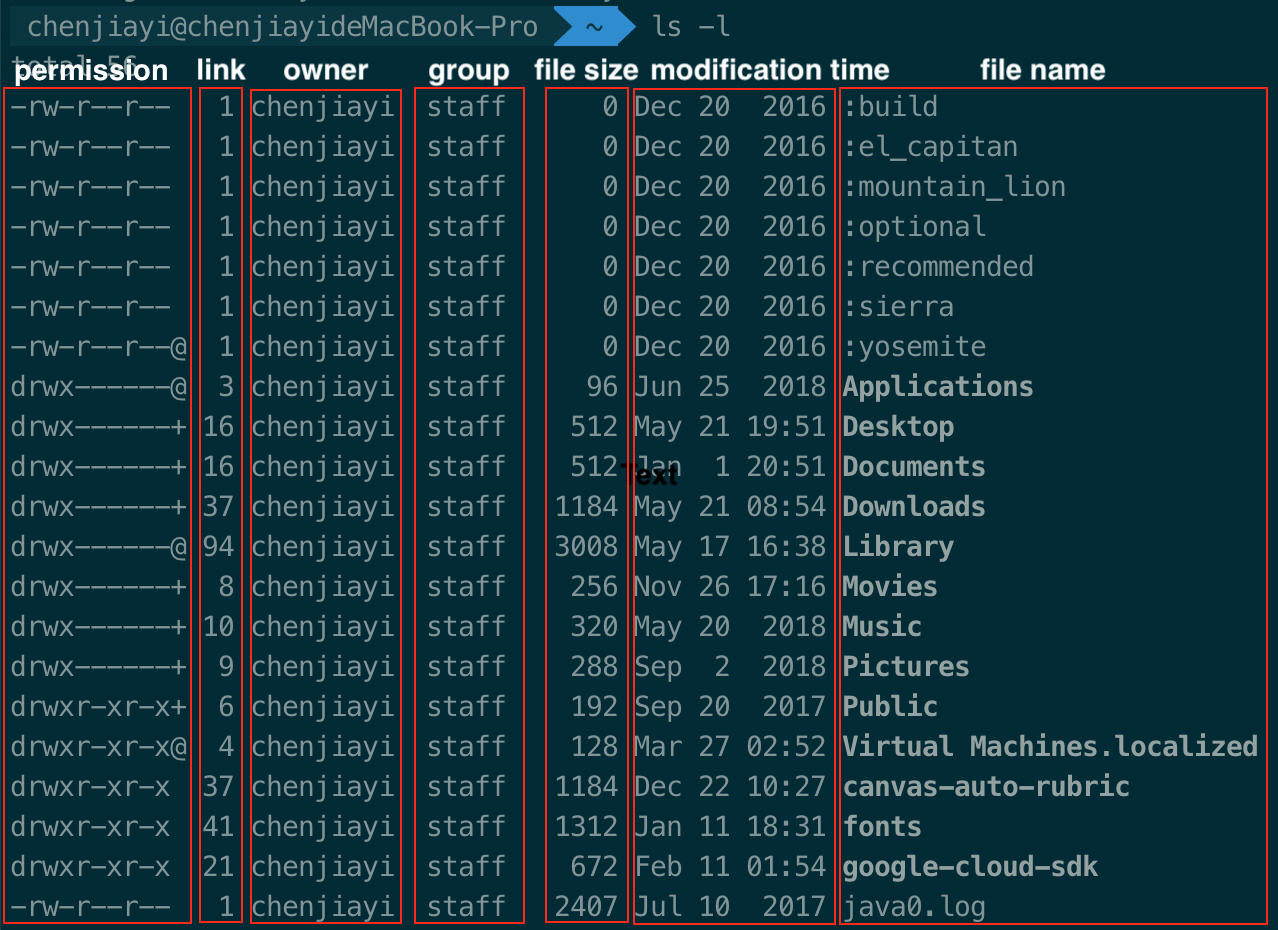
\includegraphics[width=1.1\linewidth]{fig/rc2_longformat}
	\end{figure}
\end{frame}

\begin{frame}{Aspects of Linux: Shell}
\framesubtitle{Long Format of File Information, Cont'd}
	\begin{description}[File permission]
		\item[File permission]
		\begin{itemize}
			\small
			\item first character: `-’ regular file; `d’ directory 
			\item read, write, execution permission of the owner 
			\item read, write, execution permission of the group 
			\item read, write, execution permission of everyone else
			\item last character: `-’ regular file; `x’ executable 
		\end{itemize}
		\item[Link]
		\begin{itemize}
			\small
			\item the number of hard links of the file
			\item a regular file has only one hard link (of itself)
			\item a directory has $2+n$ hard links where $n$ is the number of its subdirectories because there are two extra links to \structure{.} and \structure{..}
		\end{itemize}
		\item[Owner/Group]
		\begin{itemize}
			\small
			\item act with file permissions
		\end{itemize}
		\item[File Size] 
		\begin{itemize}
			\small
			\item in bytes
		\end{itemize}
	\end{description}

\end{frame}


\begin{frame}{Aspects of Linux: Shell}
\framesubtitle{CLI Utilities}
\begin{description}[vi/vim]
	\item[nano] Command line file editor.
	\item[diff] Compare the \textbf{diff}erence of two files. 
	\begin{description}[-]
		\small
		\item[-y] A side by side view, try it yourself.
		\item[-w] Ignore white spaces.  
	\end{description}
	\item[less] Prints the content from its \texttt{stdin} in a readable way.
	\item[vi] Advanced text editor
	\item[vim] \textbf{v}i \textbf{im}proved, both \texttt{vi} and \texttt{vim} can be exited by first press \texttt{ESC} and type ``\texttt{:q!}". You should know this in case your ``friend" opens a \texttt{vi} window when you are away, so you won't get stuck inside.
	\item[grep] Filters input and extracts lines that contains specific content. Very useful in debugging programs. 
	\item[echo] Prints its arguments to \texttt{stdout}.
\end{description}

\end{frame}

\begin{frame}{Aspects of Linux: Shell}
\framesubtitle{IO Redirection}
When you are reading \texttt{cin} or writing to \texttt{cout}, you are essentially read/writing 2 special files. Again, abstraction, right? 

It is possible to ``switch" these two ``virtual files" with real files before the actual execution of the program. This is called IO ``redirection".

There are 4 most common redirections:

\begin{description}[\texttt{exec >> output}]
	\item[\texttt{exec < input}] Use \texttt{input} as \texttt{stdin} of \texttt{exec}
	\item[\texttt{exec > output}] Write the \texttt{stdout} of \texttt{exec}  into \texttt{output}. Note this command always truncates the file. File will be created if it is not already there.
	\item[\texttt{exec >> output}] Similar to \texttt{>}, but it appends to \texttt{ouput}.
	\item[\texttt{prog1 | prog2}] Called a ``pipe". Connects the \texttt{stdout} of \texttt{prog1} to \texttt{stdin} of \texttt{prog2}
\end{description}
\end{frame}

\begin{frame}{Aspects of Linux: Shell}
\begin{block}{Globbing}
	Sometimes you don't care about one file, you care about \textbf{all} files. You can use \texttt{*} to represent any string in command arguments. This is called ``globbing" and the \texttt{*} is called a wildcard.
	
	\begin{itemize}
	\item List every \texttt{.cpp} file in home dir: \texttt{\$ ls -al $\sim$/*.cpp}
	\item Delete everything in \texttt{/temp}: \texttt{\$ rm -rf /temp/*}
	\item Combine all \texttt{.h} into one: \texttt{\$ cat *.h > combined.h}
	\end{itemize}
\end{block}

\begin{block}{Looking for help}
	The ``goto" location for help in Linux is the \texttt{man} command. This is a short hand of ``\textbf{man}ual". 
	\begin{itemize}
		\item Find out information about ``vi": \texttt{\$ man vi}
		\item Confused about \texttt{cp}: \texttt{\$ man cp}
	\end{itemize}
\end{block}
\end{frame}

\begin{frame}[fragile]{Example of shell commands}
\framesubtitle{Setup}
	The following program \texttt{rc2xm} reads from it's standard input line by line and prepends \texttt{xm} at the beginning and print it out. 
	\inputminted{c++}{code/rc2xm/xm.cpp}
	We prepare an input file \texttt{xm.in} with the following content:
	
	\small{\texttt{xd$\hookleftarrow$ cg$\hookleftarrow$ hss $\hookleftarrow$ xtt $\hookleftarrow$ qs $\hookleftarrow$ jcc $\hookleftarrow$ xdtql $\hookleftarrow$ zdnxd $\hookleftarrow$}}
	
	We use $\hookleftarrow$ to represent new-line to save space on slides.
\end{frame}

\begin{frame}{Example of shell commands}
\framesubtitle{Examples}
For each of the following commands what is it's effect? What is the final output?
\vspace{-.2in}
\begin{columns}
	\column{.5\textwidth}
	\begin{block}{The commands}
		\texttt{\$ cat xm.in}\\
		\texttt{\$ cat xm.in > xm3.in}\\
		\texttt{\$ ./rc2xm < xm.in}\\
		\texttt{\$ ./rc2xm < xm.in > xm.out}\\
		\texttt{\$ cat xm* > xm2.in}\\
		\texttt{\$ cat xm*.in >> xm.out}\\
		\texttt{\$ cat xm* | ./rc2xm > out}\\
		\texttt{\$ ./rc2xm <out | grep "xd"}
	\end{block}
	\column{.5\textwidth}
	\begin{block}{Output of last command}
	\texttt{xmxmxmxd$\hookleftarrow$xmxmxmxdtql$\hookleftarrow$
xmxmxmzdnxd$\hookleftarrow$xmxmxd$\hookleftarrow$
xmxmxdtql$\hookleftarrow$xmxmzdnxd$\hookleftarrow$
xmxmxd$\hookleftarrow$xmxmxdtql$\hookleftarrow$
xmxmzdnxd$\hookleftarrow$xmxmxmxd$\hookleftarrow$
xmxmxmxdtql$\hookleftarrow$xmxmxmzdnxd$\hookleftarrow$
xmxmxd$\hookleftarrow$xmxmxdtql$\hookleftarrow$
xmxmzdnxd$\hookleftarrow$xmxmxd$\hookleftarrow$
xmxmxdtql$\hookleftarrow$xmxmzdnxd$\hookleftarrow$}
	\end{block}
\end{columns}
\end{frame}

\begin{frame}{An extra story: Package Managers}
\begin{block}{The need for a package manager}
	\begin{itemize}
		\item Packages a fancy name for "a piece of software"
		\item Linux fs convention separates package into different locations.
		\item Packages reuse code from other packages, i.e. \textit{dependencies}.
	\end{itemize}
\end{block}
\begin{block}{The \texttt{apt} package manager}
	\begin{itemize}
		\item Standard choice for Debian (and its derivatives)
		\item \texttt{apt-get install} for installing new package.
		\item \texttt{apt-get upgrade} for upgrading existing package.
		\item \texttt{apt-get update} refreshes the list of available software.
		\item \texttt{apt-get autoremove} removes installed package.
		\item \texttt{apt moo} for a tiny surprise :)
	\end{itemize}
\end{block}
\end{frame}




	\section{RC Week 3}
\subsection{Building a C++ program}
\begin{frame}{The problem of \textit{building} complex programs}
\vspace{-0.10in}
\begin{block}{\textit{Building} is different from \textit{compiling}}
	\vspace{-0.07in}
	\begin{itemize}
		\item Compiling refers to the process of translating code to binaries.
		\item Building is \textbf{piecing together} from its components.
		\item A program might depend on other package.
		\item A program might use a pre-compiled library.
		\item A program might involve more than one source files.
		\item A program might need to be built for different platform
		\item Sometimes you not only needs to build just one executable, but also documentations / test suites / libraries for the sake of other programs.
	\end{itemize}
\end{block}
\vspace{-0.15in}
\begin{block}{How complicated is Linux kernel version 3.2?}
	\vspace{-0.07in}
	\begin{itemize}
		\item 37,626 – The number of files 
		\item 15,004,006 – The number of lines of code 
	\end{itemize}
\end{block}
\end{frame}

\begin{frame}{\textit{Building} a multi-file C++ program}
\begin{block}{The golden rule}
	\vspace{0.05in}
	\textrm{\textbf{\large{Each source file (\texttt{.cpp}, \texttt{.c}) compiles independently.}}}
\end{block}
\begin{block}{The \textit{building} process}
	\vspace{0.1in}
	\centering

	% Define block styles
	\tikzstyle{decision} = [diamond, draw, fill=blue!20, 
	text width=4.5em, text badly centered, node distance=3cm, inner sep=0pt]
	\tikzstyle{block} = [rectangle, draw, fill=blue!20, 
	text width=5em, text centered, rounded corners, minimum height=4em]
	\tikzstyle{line} = [draw, -latex']
	\tikzstyle{cloud} = [draw, ellipse,fill=red!20, node distance=3cm,
	minimum height=2em]
	
	\begin{tikzpicture}[node distance = 3cm, auto, scale=0.8, every node/.style={scale=0.8}]
	% Place nodes
	\node [block] (source) {Source \texttt{.cpp}};
	\node [draw,trapezium,trapezium left angle=70,trapezium right angle=-70, above of=source, node distance=2cm] (preproc) {Preprocessor};
	\node [block, above of=preproc, node distance=2cm] (prep) {Preprocessed Source \texttt{.cpp}};
	\node [draw,trapezium,trapezium left angle=70,trapezium right angle=-70, right of=prep, node distance=3cm] (compiler) {Compiler};
	\node [block, right of=compiler] (object) {Objects files \texttt{.o}};
	\node [block, below of=object] (outside) {Other Objects \texttt{.o}};
	\node [draw,trapezium,trapezium left angle=70,trapezium right angle=-70, right of=object] (linker) {Linker};
	\node [block, right of=linker] (executable) {exactuable};
	%\node [block, below of=decide, node distance=3cm] (stop) {stop};
	% Draw edges
	%\path [line] (source) -- (compiler);
	\path [line] (source) -- (preproc);
	\path [line] (preproc) -- (prep);
	\path [line] (prep) -- (compiler);
	\path [line] (compiler) -- (object);
	\path [line] (object) -- (linker);
	\path [line] (outside) -- (linker);
	\path [line] (linker) -- (executable);
	\end{tikzpicture}
\end{block}
\end{frame}

\begin{frame}{The \texttt{g++} tool chain}
\begin{block}{\texttt{g++} as a all-in-one tool}
	\vspace{-0.07in}
	\begin{itemize}
		\item Preprocessor, compiler and linker used to be separate.
		\item Now \texttt{g++} combines them into one.
		\item By default \texttt{g++} takes source files and generate executable.
		\item Using different switches you can perform individual step.
	\end{itemize}
\end{block}
\vspace{-0.15in}
\begin{block}{Options for \texttt{g++}}
	\vspace{-0.07in}
	\begin{description}[-O\{0123\}]
		\small
		\item[-o out] Name the output file as \texttt{out}. Outputs \texttt{a.out} if not present.
		\item[-std=] Specify C++ standard. Recommend \texttt{-std=c++11}.
		\item[-Wall] Report all warnings.
		\item[-O\{0123\}] Optimization level. \texttt{-O2} is the recommended for release.
		\item[-c] Only compiles the file (Can not take multiple arguments).
		\item[-E] Only pre-processes the file (Can not take multiple arguments).
	\end{description}
\end{block}
\end{frame}

\begin{frame}[fragile]{An example}
This example contains a ``main" source file accompanied with multiple other source files. All files are compiled separately into object files. We link some of them together and see what happens.

\vspace{0.04in}
\textit{Keep in mind variables/function must be first declared before used.}

\vspace{0.04in}
\texttt{$-->$ code/rc3build/main.cpp}
\inputminted{c++}{code/rc3build/main.cpp}
\end{frame}

\begin{frame}[fragile]{An example}
\label{example:dec_def}
\vspace{0.04in}
\texttt{$-->$ code/rc3build/odd.cpp}
\inputminted{c++}{code/rc3build/odd.cpp}

\vspace{0.04in}
\texttt{$-->$ code/rc3build/even.cpp}
\inputminted{c++}{code/rc3build/even.cpp}

\vspace{0.04in}
\texttt{$-->$ code/rc3build/sum.cpp}
\inputminted{c++}{code/rc3build/sum.cpp}
\end{frame}

\begin{frame}[fragile]{An example}
\texttt{$-->$ code/rc3build/prod.cpp}
\inputminted{c++}{code/rc3build/prod.cpp}

\vspace{0.04in}
\begin{small}
	The following file is a C source file. This file is given just for you to know you can do pretty weired things if you know the deal.
\end{small}

\texttt{$-->$ code/rc3build/sum\_large.c}
\inputminted{c++}{code/rc3build/sum_large.c}

\end{frame}

\begin{frame}[fragile]{An example}
We compile the source files one by one. 
\begin{minted}{text}
$ g++ -o main.o -c main.cpp
$ g++ -o odd.o -c odd.cpp
$ g++ -o even.o -c even.cpp
$ g++ -o sum.o -c sum.cpp
$ g++ -o prod.o -c prod.cpp
\end{minted}
Next one is compiled through gcc
\begin{minted}{text}
$ gcc -o sum_large.o -c sum_large.c
\end{minted}

Next step we are going to link (some of) them and execute it. Linking in \texttt{g++} is easy. If you supply \texttt{.o} files, \texttt{g++} will know that is should link them instead of compiling them.

Pay extra attention to compiler errors (actually linker errors), they are the most interesting part.

\end{frame}

\begin{frame}[fragile]{An example}
Now first standard examples
\begin{minted}{text}
$ g++ -o main main.o even.o sum.o && ./main
$ g++ -o main main.o even.o prod.o && ./main
$ g++ -o main main.o odd.o prod.o && ./main
\end{minted}

Now what if we link both \texttt{even.o} and \texttt{odd.o}
\begin{minted}{text}
$ g++ -o main main.o odd.o even.o prod.o && ./main
\end{minted}

Now what if we link both \texttt{prod.o} and \texttt{sum.o}
\begin{minted}{text}
$ g++ -o main main.o odd.o sum.o prod.o && ./main
\end{minted}

Now what if we leave out both \texttt{even.o} and \texttt{odd.o}
\begin{minted}{text}
$ g++ -o main main.o prod.o && ./main
\end{minted}

Now what if we leave out the \texttt{main.o} 
\begin{minted}{text}
$ g++ -o main even.o prod.o && ./main
\end{minted}

\end{frame}

\begin{frame}[fragile]{An example}
\framesubtitle{Surprises}

Now we introduce something crazy. The name of the function in \texttt{sum\_large.c} is really strange. But we just ignores that link its object file any way.
\begin{minted}{text}
$ g++ -o main main.o even.o sum_large.o && ./main
\end{minted}

Well it worked. The question is how on earth can this work. In fact \texttt{g++} is doing some crazy renaming when compiling your source code. The reason why they did this is understandable when you think about it in the later period of the course. 

Understanding linking actually allows you to do some crazy things. Try compiling the following file (with only one line of code) on your machine. 
\begin{minted}{text}
int main[-1u] = {1};
\end{minted}

It tooks quite long to finish. How large is the executable?

\end{frame}

\begin{frame}{Headers and inclusion}
\begin{block}{\texttt{\#include<>} : Why we need them?}
	\begin{itemize}
		\item Things must be declared before used.
		\item Each source file compiles independently. Needs a method to ``export" functions defined in one file to other files.
		\item Avoid repeating declarations. 
	\end{itemize}
\end{block}
\begin{block}{Preprocessing}
	\begin{itemize}
		\item Preprocessing is purely \textbf{textual}. 
		\item \texttt{\#include} simply copy the content.
		\item \textit{Conditional compilation directives }simply deletes unused branch. (\texttt{\#ifdef}, \texttt{\#ifndef}, \texttt{\#else}, ...)
	\end{itemize}
\end{block}

\end{frame}

\begin{frame}[fragile]{Header guards}
\framesubtitle{problem}
Whenever there is dependence of source files, there will be dependence of headers.

Consider the following \texttt{a.cpp}, \texttt{a.h}, \texttt{b.h} and \texttt{c.h}. Keep in mind that \textit{everything in C++ is allowed to have at most 1 definition during compilation.}

\begin{columns}
	\column{.5\textwidth}
	$-->$ \texttt{a.cpp}
\begin{minted}{c++}
#include "a.h"
#include "b.h"
int main() {...}
\end{minted}
	\column{.5\textwidth}
$-->$ \texttt{point.h}
\begin{minted}{c++}
struct Point{
    int x, y;
}
\end{minted}
\end{columns}
\vspace{0.2in}
\begin{columns}
	\column{.5\textwidth}
	$-->$ \texttt{a.h}
\begin{minted}{c++}
#include "point.h"
int area(Point a, Point b);
\end{minted}
\column{.5\textwidth}
$-->$ \texttt{b.h}
\begin{minted}{c++}
#include "point.h"
void circle(Point o, int r);
\end{minted}
\end{columns}
\end{frame}

\begin{frame}[fragile]{Header guards}
\framesubtitle{Solution}
The idea is to use a unique macro to guard a header.
\begin{itemize}
	\item Define that unique macro when the header is first included.
	\item Check if the macro is defined in future inclusion.
\end{itemize}

Now \texttt{point.h} becomes:

\begin{minted}{c++} 
#ifndef _POINT_H_
#define _POINT_H_
struct Point {int x, y;}
#endif
\end{minted}

The macro could be something else. Just don't use something common.

\end{frame}

\begin{frame}{Build systems}
\structure{The need for a build system}
\begin{itemize}
	\item Build process is complicated, avoid type every command.
	\item Project have dependence, need to manage dependence
	\item Compile minimum amount of code possible upon update.
	\item Many other reasons, abstract out actual compiler, compile for different platform / target.
\end{itemize}
\structure{Choices of build systems}
\begin{description}[GNU/make]
	\item[GNU/make] Our choice of make system. It has a very long history.
	\item[CMake] A modern make system used by CLion and many other projects. Very flexible and reliable. It is also a cross platform solution.
	\item[MSBuild] Build system used by Visual Studio.
\end{description}
\end{frame}

\begin{frame}{\textit{Makefile} and it's syntax}
\structure{The \textit{Makefile}}
\begin{itemize}
	\item The executable for GNU/make is simply \texttt{make}
	\item \texttt{make} requires a file that describes the building process. Such file is named \texttt{Makefile}. 
	\item \texttt{Makefile} is made up of \textit{targets}. A target can depend on other target, or some file.
\end{itemize}
\structure{Syntax}

The following syntax defines a target. Note the \texttt{tab} key.

\vspace{0.1in}

\texttt{\textit{TargetName} : Dep1 Dep2 file1.o file2.o}

\texttt{\keys{\tab} \textit{Command1-to-run}}

\texttt{\keys{\tab} \textit{Command2-to-run}}

\end{frame}

\begin{frame}{\textit{Makefile} : Example}
This is a \texttt{Makefile} for our previous example.
\texttt{$-->$ code/rc3build/Makefile}
\inputminted{c++}{code/rc3build/Makefile}
\end{frame}

\subsection{Misc of C++}
\begin{frame}{Standardized C++}
Once upon the time, programming languages are just conventions, design choices made by the language creator. 

\structure{The standardize process}
\begin{itemize}
	\item Establishes program syntax, what are acceptable and what are syntax errors?.
	\item Language semantics, what's the ``meaning" of an expression / language construct.
	\item Behavior, what are the expected behavior and what are undefined and left to the choice of compilers ...
	\item Standard library, what to include and what's the implementation constraint.
\end{itemize}
The latest standard is C++17 (3/21/2017). Major standards are C++98, C++03, C++11, C++14. C++ after C++11 is generally considered ``modern C++". 
\end{frame}

\begin{frame}{Online reference for \texttt{std::to\_string()}}
The following information comes from \texttt{http://www.cplusplus.com/reference/string/to\_string/}
\begin{figure}
	\centering
	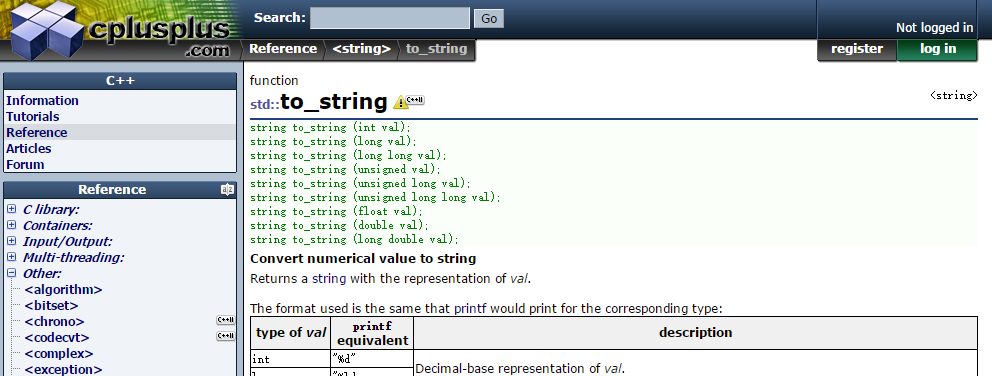
\includegraphics[scale=0.4]{fig/rc3_tostring}
	\caption{Online reference for \texttt{C++11} library function \texttt{to\_string}}
	\vspace{-0.2in}
\end{figure}

\begin{itemize}
	\item Notice the \texttt{C++11} sign.
	\item Notice the overloads supported by this function.
\end{itemize}
\end{frame}

\begin{frame}{\textit{Undefined Behaviors}}
One outcome from the standardize process is that, almost every true-or-false question about the C++ program can be answered with one of the following decisively. It is either YES, NO, or more importantly \textbf{undefined behavior} (\textit{UB} for short).

Undefined behaviors are program whose output depends on a specific platform, or a specific implementation of the compiler. You should always remember the following:
\begin{itemize}
	\item It's an absolute waste of time trying to figure out what will happen given an code that contains UB.
	\item It's dangerous and to write code that contains UB.
	\item Anyone who test you with UB, is both stupid and ignorant.
\end{itemize}

There is a reason why UB exists. It's not that the committee doesn't know how to eliminate them, but they leave room for pretty impressive \textit{compiler optimizations}.
\end{frame}

\begin{frame}{Undefined Behaviors}
Any (zero or more) of the following may happen if you trigger any of undefined behaviors:

\begin{itemize}
	\item The compiler may refuse to compile.
	\item The compiler still compiles, but throw you an warning
	\item The compiler compiles silently.
	\item Your program crashes when executed.
	\item Your program malfunctions when executed.
	\item The compiler deletes all your photos.
	\item 72 fairies come out of your screen and dance around you.
	\item \textbf{\textcolor{red}{Your program works perfectly.}}
\end{itemize} 

\textbf{It's your job to avoid UB}. We may refuse to answer the ``why my program works locally but crashes on OJ" type of question.
\end{frame}

\begin{frame}[fragile]{Undefined Behaviors}
\framesubtitle{dCommon cases}


- Integer overflow (No, it's not guaranteed to be negative!)
\begin{minted}{c++}
int x = INT_MAX; x++; 
\end{minted}

- Dereferencing \texttt{nullptr} (No, it's not guaranteed to be crash!)
\begin{minted}{c++}
int* x = nullptr; *x = 2;
\end{minted}

- Array out-of-bound (Even taking address is UB!)
\begin{minted}{c++}
int x[10] = {0};  x[10] = 1; int* x = &(x[11]);
\end{minted}



- Dangling references (You could still get correct value)
\begin{minted}{c++}
int* x = int[10]; x[3] = 5; delete[] x; cout << x[3]; 
int* f(int t) {return &t;} int* x = f(10); cout << *x;
\end{minted}

- Evaluation order and side effect :)
\begin{minted}{c++}
int i = 0; i = i++; // Yes that's UB
int j = i++ + ++i; // Yes that's UB too
f(j = i, i = j); // That's right UB again.
\end{minted}

\end{frame}

\begin{frame}{\textit{Declaration} versus \textit{Definition}}
	This whole discussion is based on one fact. 
	\begin{itemize}
		\item C++ is \textit{statically typed}
		\item Type of every identifier must be known when used.
		\item This ``identifier" includes functions, variables and arrays ...
		\item However the actual implementation can be specified later.
		\item A \textit{declaration} is a statement about what the type of an identifier (variable / function) is. 
		\item A \textit{definition} is a statements about what that object actually is. That is how much memory it consumes, what's it's data.
	\end{itemize}
	
	You have met declarations and definitions in Page.\ref{example:dec_def}.
	\texttt{extern int numbers[];} and \texttt{int reduce(int n[], int s);} are examples of declarations. The actual definition is in another file.
	
	The \texttt{extern} keyword, why is it there? 
\end{frame}

\begin{frame}[fragile]{Function \textit{signature} / \textit{prototype} and \textit{definition}}
A declaration for a function is called a function prototype. The ``type" of a function is called it's \textit{signature}. (Technically the ``signature" is not the ``type", but that's the idea.)

How much information do you need to describe the function?
\begin{itemize}
	\item The name, we need to be able to refer to that function
	\item Return type, the ``codomain" of the function.
	\item Number of inputs and their type. ``domain" of the function.
	\item Formal parameter name.
\end{itemize}

Combining them, the standard form of a function declaration will be:
\begin{minted}{c++}
ReturnType functionName(T1 arg1, T2 arg2, ...);
\end{minted}
I guess you are quite familiar with it. Note a definition of a function automatically introduce it's declaration (so the rule that everything must be declared before used is still intact).
\end{frame}

\begin{frame}[fragile]{Example}
Now a really simple example. Consider writing a declaration for the following \texttt{add} function.
\begin{minted}{c++}
int add(int x, int y) {return x + y;}
\end{minted}
No doubt above is a function definition. We first write
\begin{minted}{c++}
int add(int x, int y);
\end{minted}
Well, that's a right answer. But we could also do
\begin{minted}{c++}
int add(int elephant, int haskell);
\end{minted}
Suprised? Well it makes sense since changing formal arguments doesn't change the function at all! $f(x) = x$ and $f(z) = z$ are the same function. But we could push this even further!
\begin{minted}{c++}
int add(int, int);
\end{minted}
This will work as well, Why? This kind of declaration will be useful when you learn about function pointers.
\end{frame}

\begin{frame}[fragile]{\textit{lval} and \textit{rval}}
Compare the following 2 expression, suppose \text{arr} is an array of integers
\begin{enumerate}
	\item \mintinline{c}{arr[10]}
	\item \mintinline{c}{arr[10] + arr[1]}
\end{enumerate}
They both have the type \texttt{int} of course. 
\begin{itemize}
	\item \mintinline{c}{int *p = &(arr[10]);} makes sense.
	\item \mintinline{c}{int *p = &(arr[10] + arr[1]);} gives you compile error.
\end{itemize}  
Further more
\begin{itemize}
	\item \mintinline{c}{arr[10] = 10;} makes sense.
	\item \mintinline{c}{arr[10] + arr[1] = 20;} doesn't
\end{itemize} 
Clearly the two expression are ``different" in some sense. How? Think about memory! The first kind is called \textit{left values} and the second is called \textit{right values}. (Those are not technical definitions.)
\end{frame}

\begin{frame}[fragile]{References}

\textit{What we discuss here applies only to non-const references!}

Lvals always corresponds to a fixed memory region. This gives rises to a special construct called \textit{references}. 

\begin{minted}{c++}
int a = 1, b[10] = {2};
int& ra = a; int& rb3 = b[3];
a = 10; /* ra reads 10 */ ra = 20; // a reads 20
\end{minted}

Think about references as aliases. Essentially, you are giving the memory region associated with \texttt{a} an extra name \texttt{ra} (memory region given by \texttt{b[3]} an extra name \texttt{rb3}). 

Try resist the temptation to think reference as an \textbf{alias of variables}, but remember they are alias for the \textbf{memory region}.

References must be \textit{bind} to a memory region when created. There is no way to \textit{re-bind} of an existing reference. 
\end{frame}

\begin{frame}[fragile]{Function argument passing}
Syntacticly there exists 2 ways of argument passing:

\structure{Pass-By-Value}
\begin{minted}{c++}
int f(int x) { return (x = 2);}
\end{minted} 

\structure{Pass-By-Reference}
\begin{minted}{c++}
int g(int& x) { return (x = 2);}
\end{minted} 

We give the following code to demonstrate their difference:
\begin{minted}{c++}
int y = 10; f(y); cout << y; // returns 2, outputs 10
int z = 10; g(z); cout << z; // returns 2, outputs 2
\end{minted}
From a language point of view, reference parameter allows the function to change the input parameter. 

Some would argue there exists a third way of argument passing. 
\begin{minted}{c++}
#define SQR(x) (x * x)
\end{minted}
They have a point. We call this pass-by-name. But we choose to ignore that in this course.

\end{frame}

\begin{frame}[fragile]{Function argument passing}
Remember we are discussing how C++ manages memory. Keep in mind a memory oriented point of view is of utter importance.

We comment these two in terms of memory:
\begin{itemize}
	\item Using the pass by reference, the formal argument would be a reference to the actual argument, namely they refer to the same memory region.  
	\item Using the pass-by-value, the formal argument would be an independent \textit{copy} of actual argument. 
\end{itemize}

Pass-by-reference sounded like that it is related to pointers. This is true, in many implementations, pass-by-reference is implemented through pointers.

In pass-by-value, the word ``copy" is extremely interesting. The fact that we need to ``copy" the argument, give rise to serious problems in the later sections of this course. 
\end{frame}

\begin{frame}{Function argument passing}
This memory point of view discussion give rise to some argument:
\begin{itemize}
	\item Reference introduce an extra layer of indirect access to the original memory object, which drags down the performance.
	\item Pass-by-value needs to copy the argument, which can be slow.
\end{itemize}

In light of these observation, we suggest the following:

\begin{itemize}
	\item Small types (\texttt{int}, \texttt{float}, \texttt{char*}...) better passed by value. The cost of indirect access is much more than copying them.
	\item Complicated structure, especially large ones, or class object, better passed through reference.
\end{itemize}

On the other hand, references allows the function to change the parameter, and sometimes would like to enforce invariance of arguments. This will be solved later.
\end{frame}

\begin{frame}[fragile]{Memory layout for \textit{array} and \textit{struct}}
\begin{columns}
	\column{.5\textwidth}
	\structure{Array}
	
	Arrays are arranged in a consecutive way in memory. 
	
	Consider \texttt{int x[6];}. Each \texttt{int} costs 4 bytes. 

\vspace{.2in}
\begin{bytefield}[leftcurly=., leftcurlyspace=0pt]{16}
	\bitheader[endianness=little]{0,4,8,12}\\
	\begin{leftwordgroup}{0x90}
		\bitbox{16}{Random data...}
	\end{leftwordgroup}\\
	\begin{leftwordgroup}{0xA0}
		\bitbox{4}{\texttt{x[0]}}\bitbox{4}{\texttt{x[1]}}
		\bitbox{4}{\texttt{x[2]}}\bitbox{4}{\texttt{x[3]}}
	\end{leftwordgroup}\\
	\begin{leftwordgroup}{0xB0}
		\bitbox{4}{\texttt{x[4]}}\bitbox{4}{\texttt{x[5]}}
		\bitbox{8}{Unknown}
	\end{leftwordgroup}\\
	\begin{leftwordgroup}{0xC0}
		\bitbox{16}{Random data...}
	\end{leftwordgroup}\\
\end{bytefield}
Note \texttt{x[i]} is always \texttt{*(x + i)}. \texttt{x} essentially holds address \texttt{0xA0}.\\

	\column{.5\textwidth}
	\structure{Structures}
	
	\textit{\small{Warning: C++ standard does not fully specify memory layout.}}
	
	Consider a structure (32bit)
\begin{minted}{c++}
struct S {
    int x, y, z; long long l1;
    S* ptr; int t[2]; 
    long long l2;
};
\end{minted}

\begin{bytefield}[leftcurly=., leftcurlyspace=0pt]{16}
	\bitheader[endianness=little]{0,4,8,12}\\
	\begin{leftwordgroup}{0xA0}
		\bitbox{4}{\texttt{x}}\bitbox{4}{\texttt{y}}
		\bitbox{4}{\texttt{z}}\bitbox{4}{-}
	\end{leftwordgroup}\\
	\begin{leftwordgroup}{0xB0}
		\bitbox{8}{\texttt{l1}}\bitbox{4}{\texttt{ptr}}
		\bitbox{4}{t[0]}
	\end{leftwordgroup}\\
	\begin{leftwordgroup}{0xC0}
		\bitbox{4}{\texttt{t[1]}}\bitbox{4}{-}\bitbox{8}{\texttt{l2}}
	\end{leftwordgroup}\\
\end{bytefield}
\end{columns}
\end{frame}

\begin{frame}[fragile]{Remarks on arrays}
Arrays are passed by passing the address of its first element. That \textbf{address is copied}, in this sense the actual content of the array is passed as references. 



You might wonder the difference of the following 2: 

\begin{minted}{c++}
int foo(int x[], int size);
int foo(int *x, int size);
\end{minted}

In practice there aren't any (if not templates).

Remember the following expression does \textbf{NOT} make sense:
\begin{minted}{c++}
int foo(int x[size]);
\end{minted}

Whenever you need to pass an array as an argument, remember to \textbf{pass it's size along with it}! 

\small{Footnote: In fact C++ considers the size of the array part of its type, meaning C++ believes for \texttt{int x[3];} and \texttt{int y[4];}, \texttt{x} and \texttt{y} has different type. It's just happens that both types can be converted into \texttt{int*} when passed as argument. See \texttt{code/rc3arr/run.sh}}
\end{frame}

\begin{frame}{Remarks on structures}
\begin{itemize}
	\item \texttt{sizeof} a struct is NOT the sum of \texttt{sizeof} its members.
	\item Structures arrange its members in the order of declaration.
	\item Members of a structure are put in the continuous region.
\end{itemize}

You need to think structures as a new type: structures a models a new type of data, a new concept. It is a \textbf{compound type}.

If you pass an structure by value, and if there is an array embedded in the structure, the array will be copied. This makes sense since the array is considered part of the value of the new datatype.

In C++, structures are simply ``\texttt{class}"es with one change : members of a structure are by default \texttt{public}. This implies classes follows the same set of rules in terms of memory layouts.

We omit the discussion on pointers of structure.
\end{frame}

\begin{frame}[fragile]{Initialization of Arrays}
The rules of initialization is extremely complicated in C++, this is due to two (competing) reasons:
\begin{itemize}
	\item C++ tries to keep backward compatibility with C. 
	\item C++ needs a unified modern syntax to initialize things.
\end{itemize}
This gets even more complicated if you take into account the fact that \texttt{struct}s are essentially same as \texttt{class}es. 

\textbf{These rules applies also to \texttt{new}/\texttt{new[]} operator}.

We first consider initializing an array:
\begin{minted}{c++}
int arr0[5] = {1, 2, 3, 4, 5}; 
int arr1[5] = {1, 2}; // {1, 2, 0, 0, 0};
int arr2[5] = {1}; // {1, 0, 0, 0, 0};
int arr3[5] = {0}; // {0, 0, 0, 0, 0};
int arr4[] = {1, 2, 3} // arr4[3] = {1, 2, 3}; useful!
int arr5[3]{1, 2}; // {1, 2, 0}; c++11 style;
int arr6[3]{}; // {0, 0, 0}; c++11 style;
\end{minted}
\end{frame}

\begin{frame}[fragile]{Initialization of structures}

\begin{columns}
	\column{.5\textwidth}
	Consider \texttt{struct S}:
\begin{minted}{c++}
struct S {
    int x, y;
    int arr[2];
    double d;
};
\end{minted}
You might need to specify \texttt{-std=c++11} when using these initializations.

Now think about it, how to initialize \texttt{S sarr[2];}?

	\column{.5\textwidth}
	\structure{Curly-brace enclosed initializer}
\begin{minted}{c++}
S s1 = {1, 2, 3, 4, 1.0};
S s2 = {1, 2, {3, 4}, 1.0};
\end{minted}
We recommend the second one.
	
\structure{Default constructor}
\begin{minted}{c++}
S s1{};
\end{minted}
This initializes all fields to zero.

\structure{In-place}
\begin{minted}{c++}
struct P {
    int x = 1, y = 2;  
    int arr[2] = {3 , 4}; 
    double d = 1.0;
};
\end{minted}
\end{columns}
\end{frame}

\begin{frame}[fragile]{Function arguments: pointers or references?}
We have one last question. Consider the following code:
\begin{minted}{c++}
struct S {int arr[100];};
void foo(S* s); void bar(S& s):
\end{minted}
Now two functions are functionally same, which should I perfer?

\begin{itemize}
	\item Pro-ref: References guarantees non-\texttt{null}, which is safer.
	\item Pro-ptr: Pointers allow \texttt{nullptr}, allows for the idea like "not-applicable" or "default value".
	\item Pro-ref: References good for \textit{ownership}, semantically clear.
	\item Pro-ref: Syntactically cleaner. No need to modify call sites.
	\item Pro-ptr: References are used like values, not intuitive. Readers of the code has to jump to decl. Example \texttt{std::getline}.
	\item Pro-ref: Pointers are easily confused with array.
	\item Pro-ptr: Pointers are the only way to work with array. (If you ignore \texttt{std::vector}).
\end{itemize}
\end{frame}

\begin{frame}{References as an abstraction}
We would like to quote the following words from the standard:
\begin{quotation}
	References are not objects; they do not necessarily occupy storage, although the compiler may allocate storage if it is necessary to implement the desired semantics.
\end{quotation}
In this way references are kind of special, since all usual types are connected to some memory: an \texttt{int} is 4 bytes and there is a 32-bit binary value in those 4 bytes. Pointer are addresses, they occupies 4 bytes in the memory and there is a 32-bit address in those 4 bytes. 

Reference is defined through \textit{abstraction}: We have a contract with the language on how this thing should behave, but we make no assumption on how the compiler achieve such effect. Compiler could choose to use pointers to achieve references, but on the other hand it doesn't have to. 
\end{frame}

\begin{frame}[fragile]{Size of a reference type}
\begin{itemize}
	\item References are often implemented by pointers.
	\item Now what is the size of the reference type.
\end{itemize}
Now \texttt{sizeof(int\&)} will not work. Std. requires \texttt{sizeof} the reference type returns \texttt{sizeof} the referenced type, \texttt{sizeof(int)}.

But we could try
\begin{minted}{c++}
struct S {int x; int& y;} cout << sizeof(S);
\end{minted}
Will this work? Consider the code on the left side. Output?
\vspace{-0.15in}
\begin{columns}
	\column{.5\textwidth}
\begin{minted}{c++}
struct S {int x; int& y};
int main() {
    int a = 3;
    S s = {a, a};
    cout << sizeof(s);
} 
\end{minted}
	\column{.5\textwidth}
	
	\structure{It could be 8}
	
	Implemented by pointers, 4 bytes.
	
	\structure{It could be 4}
	
	Compiler discovered it is not used. This also obeys the std.
	
	\structure{It could be 5, 6, 7, 9, 120. Why?}
\end{columns}
\end{frame}



	\section{RC Week 4}
\subsection{Deciphering Type Declarations}
\begin{frame}{Design choice of declarations.}
\begin{block}{Quote from \textit{The C Progamming Language}}
	\begin{quotation}
		The syntax is an attempt to make the declaration and the use agree. (In it) ... parentheses are over-used.
	\end{quotation}
\end{block}
\vspace{-.35in}
\begin{columns}
	\column[]{.33\textwidth}
	\begin{block}{Declaration}
		\begin{itemize}
			\item \texttt{int a;}
			\item \texttt{int arr[4];}
			\item \texttt{int *p;}
			\item \texttt{int *(pa[4]);\newline}
			\item \texttt{int (*pp)[4];}
		\end{itemize}
	\end{block}
	\column[]{.67\textwidth}
	\begin{block}{Intepretation}
		\begin{itemize}
			\item \texttt{a} is an \texttt{int}
			\item \texttt{arr[]}\textrightarrow \texttt{int}, \texttt{arr}\textrightarrow array of \texttt{int}
			\item  \texttt{*p}\textrightarrow \texttt{int}, \texttt{p} \textrightarrow pointer to \texttt{int}
			\item \texttt{*(pa[4])}\textrightarrow \texttt{int}, \texttt{pa[4]}\textrightarrow pointer to \texttt{int},  \texttt{pa}\textrightarrow array of pointer to \texttt{int}.
			\item \texttt{*pp} \textrightarrow array of \texttt{int}, \texttt{pp} \textrightarrow pointer to array of \texttt{int}.
		\end{itemize}
	\end{block}
\end{columns}
\end{frame}

\begin{frame}[fragile]{\texttt{const} modifier}
Whenever a type something is \texttt{const} modified, it is declared as ``immutable". Example:

\begin{minted}{c++}
const int a = 10; a = 2; // Compile error
struct P {int x = 1, y = 2;};
const P p; p.y = 3; // Compile error
\end{minted}

Remember this immutability is enforced by the compiler at compile time. This has a very strong implication. The compiler does NOT forbid you from doing strange things intentionally.

\begin{minted}{c++}
const int a = 10; 
int *p = const_cast<int*>(&a); // C++11 style cast
*p = 20; cout << a; // Will this output 20?
\end{minted}

Well this is actually UB. \texttt{const} is not a guarantee of immutability, it is an \textbf{intention}. It asks the compiler to look out for you, if you know you shouldn't change something.
\end{frame}

\begin{frame}{\texttt{const} and pointers}
	We now combine the previous discussions. 
	
	\begin{description}[\texttt{int *(const p)}]
		\item[\texttt{const int *p}] \texttt{*p} is of type \texttt{const int}, thus changing \texttt{*p} is illegal. However this declaration does \textbf{not} say anything about \texttt{p}, thus changing \texttt{p} is possible. 
		
		This is called \textit{pointer-to-const}.
		
		\item[\texttt{int *const p}] Equivalent to \texttt{int *(const p)}.
		\item[\texttt{int *(const p)}] This declaration essentially says if you dereference \texttt{const p}, you will get \texttt{int}. Since \texttt{int} is not quantified by \texttt{const}, you can change \texttt{*p}. However, the pointer itself, is modified by \texttt{const}, so you can change \texttt{p}.
		
		This is called \textit{const-pointer}.
	\end{description}
	
	Naturally you could have \texttt{const int *(const p)}. This declaration basically says both the pointer \texttt{p} itself and the dereferenced object (\texttt{const int}) cannot be changed.
\end{frame}

\begin{frame}{\texttt{const} and reference}
Recall that \textbf{references cannot be rebind once initialized}. The following definitions are equivalent. They are all \textit{const references}.

\begin{itemize}
	\item \texttt{const int\& iref}
	\item \texttt{(const int)\& iref}
	\item \texttt{int\& (const iref)}
	\item \texttt{const int\& (const iref)}
\end{itemize}

The second one makes the most sense, although the first one is the most commonly used. 

The second one essentially says,\texttt{iref} is a reference, or an alias to a memory region, that is protected by the \texttt{const} modifier. 
\end{frame}

\begin{frame}[fragile]{\texttt{const} reference and argument passing}
There is something special about const references:
\begin{center}
	\structure{Const reference are allowed to be bind to right values,\\ while normal references are not allowed to.}
\end{center}
Normally if a const reference is bind to a right value, the const reference is no difference to a simple const. 
\begin{minted}{c++}
int a=5; const int& r=a+1; const int c=a+1;
\end{minted}
In above example practically there is no difference between \texttt{r} and \texttt{c}.

But when you pass arguments through const references, things become a little bit different.
\begin{minted}{c++}
int foo(const ReallySuperLargeStruct& s);
\end{minted}
\vspace{-0.05in}
\begin{itemize}
	\item We are passing by reference, this avoids copying.
	\item \texttt{const} enforces immutability.
	\item \texttt{rval}s can be passed directly into it (unlike pointers).
\end{itemize}
\end{frame}

\begin{frame}[fragile]{Example}
\begin{columns}
	\column{.5\textwidth}
\begin{minted}{c++}
int foo(int); int bar(int&);
int baz(const int&);

int q = 10; int& rq = q;
const int& crq = q;
int* pq = &q; 
const int* cpq = &q;

void foobar() {
    crq = 5;   // Error!
    *cpq = 20; // Error!
    q = 30; cout << crq;  // 30
    *pq = 4; cout << *cpq // 4
}
\end{minted}
	\column{.5\textwidth}
\begin{minted}{c++}
int bazbok() {
    baz(q);   baz(20); // OK
    baz(*pq); baz(rq); // OK
	
    bar(q);   bar(*pq); // OK
    bar(10);   // ERROR
    bar(*cpq); // ERROR
    bar(crq)   // ERROR
}
\end{minted}
\end{columns}
\end{frame}

\begin{frame}[fragile]{\texttt{const} propagation and type coercion}

\begin{block}{Type coercion and type compatibility}
	You should be very familiar with types now. Types defines different kinds of things. Some of those things are \textit{compatible}, meaning one could be transformed into another implicitly. But sometimes you need to explicitly \textit{cast} them, or coerce them into another type.
		
\begin{minted}{c++}
int x = 20; long int y = 30; char* p = "hello";
y = x; /* OK */ x = y; // Compiler warning
int x = p; // Incompatible, compile error
\end{minted} 
\end{block}

	A remark is that most of the things are incompatible, simply because these different type are different from the hardware point of view. Pointers are addresses, but int are number. \texttt{long int} occupies more space than \texttt{int} etc.
	
\end{frame}

\begin{frame}[fragile]{\texttt{const} propagation and type coercion}
\framesubtitle{\texttt{const} modifier introduce incompatibility}

	The subtitle is summarized into the following rules:
	
	\begin{itemize}
		\item \texttt{const type\&} to \texttt{type\&} is \textbf{incompatible}.
		\item \texttt{const type*} to \texttt{type*} is incompatible.
		\item \texttt{type\&} to \texttt{const type\&} is \textbf{compatible}.
		\item \texttt{type*} to \texttt{const type*} is compatible.
	\end{itemize}
Example:
\begin{minted}{C++}
int foo(int& x); int bar(int* px); int cfoo(const int& x);
void baz() {
   const int *q = nullptr; int *p = q; //Compile error
   const int& r = 10;  foo(r); //Compile error
   cfoo(*p); cfoo(*q); cfoo(r); // All OK
}
\end{minted}

\end{frame}



\begin{frame}[fragile]{\texttt{const} propagation and type coercion}
\framesubtitle{\texttt{const} progagation}
Further more, \texttt{const} modifier attaches extra constrain when trying to take address or dereference / reference things.

\begin{itemize}
\item Take address of the \texttt{const} references gives pointer-to-const.
\item Dereferences pointer-to-const give const references.
\end{itemize}
Example:
\begin{minted}{C++}
int foo(int& x); int bar(int* px); int cfoo(const int& x);
void baz() {
    const int q = nullptr; int *p = &q; //Compile error
    foo(q); bar(&q)                     //Compile error
    const int& r = q; foo(r); bar(&r); // Compile errer
}
\end{minted}
This creates an important feature of C++ \texttt{const}ness:

 \structure{You either do it in full scale, or not at all}.
\end{frame}

\begin{frame}{\texttt{const} compatibility in terms of abstraction}
\small
Again I hope you could see something bigger. These rules are unlike those mentioned earlier. The compiler probably use the same representation for \texttt{type*} and\texttt{const type*}. 

They are different, because they follow different abstraction. The abstraction for \texttt{type*} supports modification, or it is supported to appear on the left hand side of the assignment operator, while the abstraction of \texttt{const type*} does not. 

This point of view also explains the propagation rules. The type system must be designed in a coherent way. If an object doesn't support modification, changing the reference to pointer won't suddenly equip it with modification. The abstraction must be maintained between operations.

This gives a very first look over the abstraction point of view of the concept ``datatype". Now we see that datatype not just the memory layout of objects, but more about abstraction, operations that the type supports.

\end{frame}



\begin{frame}{Functions Pointers: Why Pointers?}

	\structure{The Von Neumann View of functions}
	
	Functions are code, and code when compiled are simply binary number, i.e. data. The action of calling a function is simply pumping these binary numbers into the CPU (after you take VE370 you would find it's actually the other way around).
	
	\begin{itemize}
		\item Functions are just a bunch of numbers in the memory
		\item We could refer to the function by refering to the numbers
		\item These numbers has an \textit{address} (think of arrays)
		\item We could use that address to refer to the function
	\end{itemize}
	
	Variable that stores the address of functions are called \textit{function pointers}. By passing them around we could pass functions into functions, return them from functions, and assign them to variables. 
\end{frame}

\begin{frame}{Functions Pointers: Type}
But there is one question, what is the type of them? 

Well by our previous understanding dereferencing a function pointer should give us a function, just like dereferencing \texttt{int*} gives us \texttt{int}. We would like to do a comparison:

\vspace{-.2in}
\begin{columns}
	\column[]{.5\textwidth}
	\begin{block}{Function decl. \texttt{foo}}
		\begin{itemize}
			\item \texttt{void foo();}
			\item \texttt{int foo(int x, int y);}
			\item \texttt{int foo(int, int);}
			\item \texttt{int *foo(int, char*);}
			\item \texttt{char* foo(int[], int);}
		\end{itemize}
	\end{block}
	\column[]{.6\textwidth}
	\begin{block}{Function pointer \texttt{bar}}
		\begin{itemize}
			\item \texttt{void (*bar)();}
			\item \texttt{int (*bar)(int, int);}
			\item \texttt{int (*bar)(int, int);}
			\item \texttt{int *(*bar)(int, char*);}
			\item \texttt{char *(*bar)(int[], int);}.
		\end{itemize}
	\end{block}
\end{columns}
Note \texttt{int *bar(int);} does \textbf{NOT} declare a function pointer. The grouping is \texttt{int *(bar(int))}, which is declaring a function. This is related to the operator precedence of C++.
\end{frame}

\begin{frame}[fragile]{Functions Pointers: Usage}
\begin{block}{Assignment from functions}
	In fact, the identifier (name) of the functions are actually values of function pointers. 
\begin{minted}{c++}
int max(int x, int y) { return x > y ? x : y;}
int (*cmp)(int, int) = max;
\end{minted}
\end{block}
\vspace{-0.1in}
\begin{block}{Invoking a function pointer}
	You can invoke a function pointer by applying operator \texttt{()} to it.
\begin{minted}{c++}
int m = cmp(10, 20); // No need to dereference it
\end{minted}
\end{block}
\vspace{-0.1in}
\begin{block}{Invariance under \texttt{*}}
	Dereferencing a function pointer still gives back a function pointer.
\begin{minted}{c++}
int m = cmp(10, 20); // 20
int n = (*cmp)(10, 20); // 20
int p = (*******cmp)(10, 20) // 20
\end{minted}
\end{block}
\end{frame}

\begin{frame}[fragile]{Example}
The following code implements a simple calculator. Notice how function pointer helps to clarify the code.

\texttt{$-->$ code/rc4fptr/fptr.cpp}
\inputminted{c++}{code/rc4fptr/fptr.cpp}
\end{frame}


\begin{frame}[fragile]{\texttt{typedef} storage modifier}
The \textbf{typedef} keyword is actually a storage modifier (like \texttt{static}), means it goes to wherever \texttt{static} can appear. 

Reading a \texttt{typedef} is actually very simple:
\begin{enumerate}
	\item Ignore \texttt{typedef} and read the line as if it is a real declaration.
	\item Now the ``declared" variable would have a declared type
	\item Finally we put back \texttt{typedef}. The variable now become an alias to the declared type.
\end{enumerate}
Example:
\begin{minted}{c++}
typedef bool (*comparator)(double, double);
typedef const Comparator const_comparator;
const_comparator *p = nullptr;
*p = min; // Error!, p is pointer-to-const
comparator cmp[] = {min, max}; // Array of function ptrs
\end{minted}
\end{frame}


\begin{frame}[fragile]{Semantic of \texttt{typedef}}
\framesubtitle{Motivation}
It is now to analyze the semantic of \texttt{typedef}: not how is used, but why is it used in such way. If you go through the standard library. you would find some code like:
\begin{minted}{c++}
typedef unsigned int size_t;
\end{minted}
What's the point of doing this if when you can just use \texttt{unsigned int }? Suppose you are trying to find your name with your student ID, which is an unsigned integer:
\begin{minted}{c++}
string getNameByID(unsigned int student). 
\end{minted}
This is not good, because \texttt{student} is not any \texttt{unsigned int}, it must be a student ID. You would like to emphasize on that:
\begin{minted}{c++}
typedef unsigned int student_id; 
string getNameByID(student_id id);
\end{minted}
\end{frame}

\begin{frame}[fragile]{Semantic of \texttt{typedef}}
But here comes a problem:
\begin{center}
	\structure{\texttt{typedef} creates alias, not new types.}
\end{center}
This essentially says both \texttt{student\_id} and \texttt{size\_t} are both alias for \texttt{unsigned int}. They are essentially considered the same thing.

The following code does not \textbf{NOT} make sense:

\begin{minted}{c++}
size_t numberOfApples = 20;
string name = getNameByID(numberOfApples);
\end{minted}

but the compiler lets you do this without even a warning. Semantic of the types should prevent you from making these assignments (easily), but \texttt{typedef} breaks this promise.

On the other hand, \texttt{classes} are more modern. Two \texttt{classes} with same ``composition" are considered incompatible different types.`

\end{frame}

\subsection{Procedure Abstraction}
\begin{frame}{Abstraction and \textit{decoupling}}
The motivation of all abstraction comes directly from the need for decoupling. We would like to design the software in such way, that the change in one portion of the code does not affect the others.

\vspace{0.1in}
But after all some degree of coupling is inevitable, conceptually we would like to limit the coupling only to the interfaces, i.e. where modules connect.

\begin{columns}
	\column{.33\textwidth}
	\structure{Low coupling:}
	\begin{figure}
		\centering
		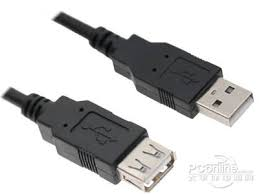
\includegraphics[scale=0.34]{fig/low-coupling}
	\end{figure}
	\column{.34\textwidth}
	\structure{High coupling:}
	\begin{figure}
		\centering
		
\includegraphics[scale=0.35]{fig/high-coupling}
	\end{figure}
	\column{.33\textwidth}
	\structure{Low coupling for flexibility:}
	\begin{figure}
		\centering
		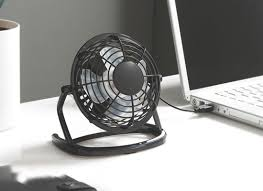
\includegraphics[scale=0.33]{fig/low-coupling-flex}
	\end{figure}
\end{columns}

\end{frame}

\begin{frame}{Independence of variation}
We some times simply refer these interfaces, or connection points, \textit{the abstraction}. Now we take a look at the \textit{implementation} side of the abstraction.

If you the abstraction implementation is done right, you should find the following property of your abstraction.

\begin{itemize}
	\item Locality. The implementation should only depend on other abstraction, not abstraction implementation.
	\item Substitutable. The implementation is not unique. Any implementation that obeys the abstraction should work.
\end{itemize}

The ultimate goal is the the only coupling point in your program should be the abstraction. \alert{So this is utterly import to always think through the abstraction before the actual implementation.}
\end{frame}

\begin{frame}{Elements in procedure abstraction}
A common point of where modules connect is function calls. But think bigger, when you say \texttt{printf("\%d", 1)}, you are requesting a service, requesting for certain operation. This idea that programs are driven by requests for operations sums up to the idea of \textit{Procedure Abstraction}. Remember functions are just one realization of the idea of Procedure abstraction, but not the only one.

We now examine how functions interact with the outside world. These things will be very important in specifying the abstraction:

\begin{itemize}
	\item Input and it's assumption
	\item Expected output, and the property of the output
	\item Impact on the environment, or side effects.
\end{itemize}
\end{frame}

\begin{frame}[fragile]{Specifying abstraction}
Typically an abstraction is specified in the following manner:
\begin{minted}{c++}
int reallyUselessFoo(int& intArg, string str);
// REQUIRES : intArg > 0, str != ""
// MODIFIES : cout, intArg, UsefulGlobalVar
// EFFECTS  : do Blah blah blah and return blah blah
\end{minted}
\begin{itemize}
	\item \textit{REQUIRE} clause and the function signature specifies the input. Number of inputs are fully specified by the signature, input range can be partially specified through type. 
	\item \textit{EFFECTS} clause and the function signature specifies  the output. The expected output is partially specified by the type of the return value. It is important to note that the function name is also part of the specification, it should clearly and concisely reflect on what the function does. 
	\item \textit{MODIFIES} clause specify side effects.
\end{itemize}
\end{frame}

\begin{frame}[fragile]{Side effects}
We have left out the term ``side effects" for now. Let's take a look at them. Think of mathematical functions, you would expect the following of them:
\begin{block}{Functions are maps}
Functions should return the same if provided same input:
\begin{minted}{c++}
(fun(x) == fun(x)) == true
\end{minted}

\end{block}
\begin{block}{Functions are stateless}
Programs should behave the same for the following two lines
\begin{minted}{c++}
int x = foo(y); int z = bar(x, x);
int z = bar(foo(y), foo(y));
\end{minted}

The following 2 lines should also be equivalent.
\begin{minted}{c++}
int x = foo(y); 
int x = foo(y); int x = foo(y);
\end{minted}

\end{block}
\end{frame}

\begin{frame}[fragile]{Side effects}
It is our intuition that all these assertions should be true. But unfortunately we can break them. Once we break these intuitions it will be very hard for programmers to keep track of program.

\structure{Through global/static variables}
\begin{minted}{c++}
int x = 3; int foo(int y) {return y + x++;}
int bar(int y) {static int x = 0; return y + x++;}
\end{minted}
\structure{Through modifying arguments}
\begin{minted}{c++}
int x = 3; int foo(int& x) {return ++x;}
\end{minted}
\structure{Involving IO}
\begin{minted}{c++}
int x = 3; int foo(int x) {cout << "Hello"; return x;}
\end{minted}

Functions are suppose to be maps, converting one value to another. In all these values the function does something else. They modify something that does not belong to them. 

These behaviors are called \textit{side effects}.
\end{frame}

\begin{frame}[fragile]{Function signature is important}
A huge amount of information is provided in the function signature. In fact we believe the following should be true:
\begin{center}
	\structure{Good code should be self explanatory.\\ Good abstraction should be self documenting.}
\end{center}
It means you should be able to guess the abstraction's usage, just by looking at it's function signature. Compare the following:
\begin{minted}{c++}
void dwcl(double a, double b, double c);
void drawCircle(Point p, double radius);
\end{minted}
It is generally considered good to 
\begin{itemize}
	\item Avoid introducing too much arguments. Pack arguments that are related into structure / classes.
	\item Avoid using acronyms in function names. You have very good editors that provides extensive support for auto-completion.
\end{itemize}
\end{frame}

\begin{frame}[fragile]{Leaky Abstractions}
Officially our discussion of procedural abstraction has ended. But I would like to make a few comments. We would like to ask:
\begin{center}
	\structure{Are there PERFECT abstractions?}
\end{center}
Perfect abstractions are abstractions that completely hides information about the implementation, a complete black box. People often need a perfect abstraction, e.g. for cryptography.

Compare the following, assume both arguments are positive:
\begin{minted}{c++}
int mul1(int x, int y) {return x * y;}
int mul2(int x, int y) {return x==0 ? 0 : y+mul2(x-1,y));}
\end{minted}
Both implementation are correct. Can we differentiate them? The second one is significantly slower than the first one. If we provide a really large input, we would be able to differentiate them by the runtime! We say we have a \textit{leaky abstraction} at our hand.
\end{frame}

\begin{frame}[fragile]{the Law of Leaky Abstractions}
the Law of Leaky Abstractions (Spolsky, 2002) says:
\begin{quotation}
	\structure{All non-trivial abstractions, to some degree, are leaky.}
\end{quotation}
How is this important? By now should be clear that the proper functionality of software (and computer system) often depends on the reliability of abstraction. But at some point, the abstraction will break. Examples:
\begin{itemize}
	\item In C/C++ iterating through large 2D array horizontally is significantly faster than vertically.
	\item \textit{L3-cache side channel attack}. Takes advantage a leaky abstraction inside the CPU to steal your ``password".
\end{itemize}
As a measure to counter this problem you sometimes see the standard not only specify a function's behavior, but also it's runtime (in terms of time complexity).
\end{frame}

\begin{frame}{Enforcing Abstraction in C++}
Another very interesting thing here is what happens if you breaks the abstraction? How abstraction is enforced in C++?
\begin{itemize}
	\item Input number and types are protected by the type system.
	\item Input But the properties of input (even?) are left unsaid.
	\item Output type and number (guarantees there exists one output if needed) is protected by the type system.
	\item Whether output fits the expected behavior is unchecked.
	\item Side effects are completely unchecked.
\end{itemize}
As you can see many things are left unchecked! Most of the checking is done by the type system. In fact, the type system plays a really important role in programming language.	The fact that C/C++ is a statically typed language is greatly complimented and provides much help in writing correct programs.
\end{frame}

\begin{frame}{Enforcing Abstraction: How far can we go?}
Here I list a couple of other language's idea. You may or may not know that language, but that's completely alright.
\begin{description}[Matlab/Python]
	\item[Matlab/Python] Dynamically typed. The type of arguments are not declared and only known at runtime.
	\item[Bash] Scripting language used by shell. Not even typed. Not even check the arguments of function called. Basically zero protection.
	\item[Haskell] A language that is statically typed. The type system is so powerful that it requires the programmer to declare not only the inputs, but also the ``side effects" (and checks them). 
	\item[COQ] A language that goes to the extreme. It not only asks the programmer to declare everything, it even requires the program to provide a proof (and checks the proof) of correctness.
\end{description}
\end{frame}
	\section{RC Week 5}
\subsection{Mechanism behind function calling}
\begin{frame}{Memory Layout}
Before function calling we would like to first give a brief introduction to the memory organization of the system
\begin{columns}
	\column{.5\textwidth}
	\vspace{0.05in}
	
	\begin{bytefield}[leftcurly=., leftcurlyspace=0pt]{16}
		\begin{leftwordgroup}{Low}
			\bitbox{16}{Text}
		\end{leftwordgroup}\\
		\begin{leftwordgroup}{}
			\bitbox{16}{Consts}
		\end{leftwordgroup}\\
		\begin{leftwordgroup}{}
		\bitbox{16}{Statics}
		\end{leftwordgroup}\\
		\begin{leftwordgroup}{High}
			\wordbox[lrt]{1}{Heap $\downarrow$} \\
			\skippedwords \\ 
			\bitbox[lrb]{16}{Stack $\uparrow$}
		\end{leftwordgroup}\\
	\end{bytefield}
	
	* This graph is up-side-down. 
	
	\column{.5\textwidth}
	\vspace{0.05in}
	\structure{Explanation}
	\begin{itemize}
	\item ``Text", just ``code"
	\item ``consts", not like \texttt{const int const}, but string literals, \texttt{"Hello world"}.
	\item ``Statics", global variables, static variables in functions. ``static" refers to lifetime.
	\item ``Heap", where you \texttt{new}.
	\item ``Stack", everything local. Arugments, return values, return addresses ...
	\end{itemize}
\end{columns}
\end{frame}

\begin{frame}[fragile]{Element in a stack}
\begin{columns}
	
	\column{.5\textwidth}
	\vspace{-0.15in}
	
	\begin{bytefield}[leftcurly=., leftcurlyspace=0pt]{16}
		\begin{leftwordgroup}{}
			\bitbox{16}{z = 4 @ foo(3)}
		\end{leftwordgroup}\\
		\begin{leftwordgroup}{}
			\bitbox{16}{x = 3 @ foo(3)}
		\end{leftwordgroup}\\
		\begin{leftwordgroup}{}
			\bitbox{16}{Ret = ?}
		\end{leftwordgroup}\\
		\begin{leftwordgroup}{\texttt{foo}}
		\bitbox{16}{RA = \&CALLS + 1}
		\end{leftwordgroup}\\
		\begin{leftwordgroup}{}
			\bitbox{16}{q = ? @ main()}
		\end{leftwordgroup}\\
		\begin{leftwordgroup}{}
			\bitbox{16}{p = 3 @ main()}
		\end{leftwordgroup}\\
		\begin{leftwordgroup}{\texttt{main}}
			\bitbox{16}{...}
		\end{leftwordgroup}
	\end{bytefield}
	\column{.5\textwidth}
	\vspace{-0.2in}
\begin{minted}{c++}
int foo(int x) {
    int z = x + 1;
    /* Here */ 
    return z + x;  
}
int main() {
    int p = 3;
    p = foo(p); // <- CALLS
    int q = 10;
}
\end{minted}
\end{columns}
\vspace{0.1in}
The stack maintains the following information
\begin{itemize}
	\item Function arguments. They are evaluated and on to the stack.
	\item Local variables (arrays). They are reserved before initialized.
	\item Return value and return address. Return address tells which instruction to pick up when the call returned.
\end{itemize}
\end{frame}

\begin{frame}{Remarks}
\begin{block}{Calling mechanism is about \textit{Abstraction}}
	Calling mechanism is designed in such way to support procedural abstraction. In order for the abstraction to work, we require
	\begin{center}
		\structure{Each function call is independent}
	\end{center}
	This is especially important if you have recursion calls.
\end{block}

\begin{block}{Calling mechanism is platform dependent}
	\begin{itemize}
		\item Calling mechanism is neither specified by standard, nor unique!
		\item Whose responsibility to manage arguments? Caller / callee?
		\item Compiler might optimize unused variables out.
		\item Compiler might use register to store information.
		\item Compiler is allowed optimize the entire stack frame out.
	\end{itemize}
\end{block}
\end{frame}

\begin{frame}{Puzzles for \alert{FFFUUUNNNNN}!}
Under standing calling stack is most useful in finding out what has gone wrong when you observe strange behavior of your program. This is very much like solving puzzles.

We now give you a few such puzzles to entertain you. Note all the code we gave you below contains \alert{undefined behaviors} so don't be surprised if you cannot reproduce this problem.

This is actually worth noting. Many undefined behaviors would cause different behavior since given different situation on the stack. 

\begin{itemize}
	\item This code works on my computer but crashed on OJ.
	\item This code crashes / malfunctions if I change unrelated things.
	\item Student: ``TA, my code can't work!". \\
	      TA\qquad: ``Can you demo? I can't reproduce your problem"\\
	      Student: ``Suddenly I can't Either! But it crashes on OJ!"
	\item This code randomly crashes.
\end{itemize} 
\end{frame}

\begin{frame}[fragile]{Puzzle 0: Why not VLA?}
\textit{Variable Length Arrays} (VLA) are arrays whose size are determined at compile time. For example in the following code \texttt{arrX} is a VLA, and \texttt{arrY} is a usual array.
\begin{minted}{c}
void foo() {int t = 20; int arrX[t * t]; int arrY[400];}
\end{minted}
But both C++ and C choose \textbf{not} to support this language feature (above code won't compile). Explain what's the underlying reason.

\pause
\begin{block}{Explanation}
What would be the impact of this feature? Variable length array will consume variable amount of memory.

If the array is a local variable. The stack frame size of the function cannot be determined in compile time. 

The need to know the size of a function's compile time stack frame size is centric in language design. 
\end{block}      `
\end{frame}

\begin{frame}[fragile]{Puzzle 1: Orders matter}
\texttt{$-->$ code/rc5pz1/a.cpp}
\inputminted{c++}{code/rc5pz1/a.cpp}
User inputed \texttt{Hello}, symptoms are:
\begin{itemize}
	\item Program crashes after printing 4 times of \texttt{Hello}.
	\item Program runs fines if change input to \texttt{Bad}.
	\item Program doesn't crash if switch \texttt{char a[4]} and \texttt{int x = 4}. But the program keeps printing \texttt{Hello}.
\end{itemize}
\end{frame}

\begin{frame}{Solution 1}
\begin{columns}
	\column{.5\textwidth}
	
	\begin{bytefield}[leftcurly=., leftcurlyspace=0pt]{16}
		\begin{leftwordgroup}{4B}
			\bitbox{16}{s.x = 4 @ foo()}
		\end{leftwordgroup}\\
		\begin{leftwordgroup}{1B}
			\bitbox{16}{s.a[0]  @ foo()}
		\end{leftwordgroup}\\
		\begin{leftwordgroup}{1B}
			\bitbox{16}{s.a[1]  @ foo()}
		\end{leftwordgroup}\\
		\begin{leftwordgroup}{1B}
			\bitbox{16}{s.a[2]  @ foo()}
		\end{leftwordgroup}\\
		\begin{leftwordgroup}{1B}
			\bitbox{16}{s.a[3]  @ foo()}
		\end{leftwordgroup}\\
		\begin{leftwordgroup}{\texttt{foo}}
			\bitbox{16}{RA = !!}
		\end{leftwordgroup}\\
		\begin{leftwordgroup}{\texttt{main}}
			\bitbox{16}{...}
		\end{leftwordgroup}
	\end{bytefield}
	
	Return address is corrupted.
	
	\column{.5\textwidth}
	
	\begin{bytefield}[leftcurly=., leftcurlyspace=0pt]{16}
		\begin{leftwordgroup}{1B}
			\bitbox{16}{s.a[0]  @ foo()}
		\end{leftwordgroup}\\
		\begin{leftwordgroup}{1B}
			\bitbox{16}{s.a[1]  @ foo()}
		\end{leftwordgroup}\\
		\begin{leftwordgroup}{1B}
			\bitbox{16}{s.a[2]  @ foo()}
		\end{leftwordgroup}\\
		\begin{leftwordgroup}{1B}
			\bitbox{16}{s.a[3]  @ foo()}
		\end{leftwordgroup}\\
		\begin{leftwordgroup}{4B}
			\bitbox{16}{s.x = !! @ foo()}
		\end{leftwordgroup}\\
		\begin{leftwordgroup}{\texttt{foo}}
			\bitbox{16}{RA = \&main + 1}
		\end{leftwordgroup}\\
		\begin{leftwordgroup}{\texttt{main}}
			\bitbox{16}{...}
		\end{leftwordgroup}
	\end{bytefield}

	Variable \texttt{s.x} is corrupted.
\end{columns}

\end{frame}

\begin{frame}[fragile]{Puzzle 2: Missing return value?}
\texttt{$-->$ code/rc5pz2/a.cpp}
\inputminted{c++}{code/rc5pz2/a.cpp}
This code is supposed to keeping squaring a number until it's greater than 100.
\begin{itemize}
	\item Program output random number if c/with \texttt{g++ a.cpp}
	\item Program always return 225 if c/with \texttt{g++ -O1 a.cpp}
	\item Program spits random number if c/with \texttt{g++ -O1 a.cpp}, if we change ``\texttt{foo(x);}" to ``\texttt{y = foo(x);}".
\end{itemize}
\end{frame}

\begin{frame}{Solution 2}
\begin{columns}
	\column{.5\textwidth}
	
	\begin{bytefield}[leftcurly=., leftcurlyspace=0pt]{16}
		\begin{leftwordgroup}{}
			\bitbox{16}{x = 225  @ foo(225)}
		\end{leftwordgroup}\\
		\begin{leftwordgroup}{}
			\bitbox{16}{Ret = 225}
		\end{leftwordgroup}\\
		\begin{leftwordgroup}{\texttt{foo}}
			\bitbox{16}{RA = \&foo(15)}
		\end{leftwordgroup}\\
		\begin{leftwordgroup}{}
			\bitbox{16}{x = 225  @ foo(15)}
		\end{leftwordgroup}\\
		\begin{leftwordgroup}{}
			\bitbox{16}{Ret = ?}
		\end{leftwordgroup}\\
		\begin{leftwordgroup}{\texttt{foo}}
			\bitbox{16}{RA = \&main}
		\end{leftwordgroup}\\
		\begin{leftwordgroup}{\texttt{main}}
			\bitbox{16}{...}
		\end{leftwordgroup}
	\end{bytefield}
	
	Without optimization
	\column{.5\textwidth}
	
	\begin{bytefield}[leftcurly=., leftcurlyspace=0pt]{16}
		\begin{leftwordgroup}{}
			\bitbox{16}{x = 225  @ foo(225)}
		\end{leftwordgroup}\\
		\begin{leftwordgroup}{}
			\bitbox{16}{Ret = 225}
		\end{leftwordgroup}\\
		\begin{leftwordgroup}{\texttt{foo}}
			\bitbox{16}{RA = \&main}
		\end{leftwordgroup}\\
		\begin{leftwordgroup}{\texttt{main}}
			\bitbox{16}{...}
		\end{leftwordgroup}
	\end{bytefield}
	
	After optimization
\end{columns}
\end{frame}

\begin{frame}[fragile]{Puzzle 2.5: Who moved my cheese?}
\texttt{$-->$ code/rc5pz25/a.cpp}
\inputminted{c++}{code/rc5pz25/a.cpp}

We observe the output to be \texttt{-1}. However we haven't changed the variable \texttt{cheese}. Who \texttt{mov}-ed my \texttt{cheese}.
\end{frame}

\begin{frame}{Solution 2.5}
\begin{columns}
	
	\column{.5\textwidth}
	\vspace{-0.2in}
	\begin{bytefield}[leftcurly=., leftcurlyspace=0pt]{16}
		\begin{leftwordgroup}{}
			\bitbox{16}{cheese = !! @ foo()}
		\end{leftwordgroup}\\
		\begin{leftwordgroup}{}
			\bitbox{16}{...}
		\end{leftwordgroup}\\
		\begin{leftwordgroup}{\texttt{foo}}
			\bitbox{16}{RA = \&main}
		\end{leftwordgroup}\\
		\begin{leftwordgroup}{}
			\bitbox{16}{arr[0][0]  @ main()}
		\end{leftwordgroup}\\
		\begin{leftwordgroup}{}
			\bitbox{16}{arr[0][1] @ main()}
		\end{leftwordgroup}\\
		\begin{leftwordgroup}{}
			\bitbox{16}{...  @ main()}
		\end{leftwordgroup}\\
		\begin{leftwordgroup}{}
			\bitbox{16}{arr[1][0]  @ main()}
		\end{leftwordgroup}\\
		\begin{leftwordgroup}{}
			\bitbox{16}{...  @ main()}
		\end{leftwordgroup}\\
		\begin{leftwordgroup}{}
			\bitbox{16}{Ret = ?}
		\end{leftwordgroup}\\
		\begin{leftwordgroup}{}
			\bitbox{16}{RA = ...}
		\end{leftwordgroup}\\
		\begin{leftwordgroup}{\texttt{main}}
			\bitbox{16}{...}
		\end{leftwordgroup}
	\end{bytefield}
	\column{.5\textwidth}
	
	\begin{itemize}
		\item The loop out-of-bound.
		\item How 2D arrays are stored.
		\item Understand how indexing works.
		\item We omit the arguments and return values of \texttt{foo} on the graph
	\end{itemize}
\end{columns}
\end{frame}

\begin{frame}[fragile]{Puzzle 3: A hijack}
For this puzzle to work you might need to turn off \textit{Address Space Layout Randomization} and set \texttt{-fno-stack-protector} in g++.

\texttt{$-->$ code/rc5pz3/a.cpp}
\inputminted{c++}{code/rc5pz3/a.cpp}

The trick is a carefully constructed input:
\begin{center}
 \texttt{voidsecretFunction2e34!2\&\&Q.\%x;"]}
\end{center}
We observe the output is \texttt{You shouldn't be here...}

The question is how does this happen, since \texttt{secretFunction} is not called at all?
\end{frame}

\begin{frame}[fragile]{Stack unwinding / unrolling}
Hope you still remember \textit{constructors} and \textit{destructors}!

When the function returns, it not only simply discards the stack space, it actually \textit{DESTROY}s the local objects, essentially calling their deconstructors. 

This is a very useful feature! We can use this feature to automatically release resources. Consider the following \texttt{File} class.

\texttt{$-->$ code/rc5unroll/file.h}
\inputminted{c++}{code/rc5unroll/file.h}
\end{frame}

\begin{frame}[fragile]{Stack unwinding / unrolling}
The following code executes utilizes the above code:
\texttt{$-->$ code/rc5unroll/a.cpp}
\inputminted{c++}{code/rc5unroll/a.cpp}
We paste the output:
\inputminted{text}{code/rc5unroll/out}
The files clean themselves up after returned. 
\end{frame}

\begin{frame}[fragile]{Stack overflow}
A final point is that in general your stack is rather small, compared to the heap.

We refer to an empirical experiment done by \textit{Bruno Haible} in 2009.

\begin{minted}{text}
- glibc i386, x86_64    7.4 MB
- Cygwin                1.8 MB
- Solaris 7..10           1 MB
- MacOS X 10.5          460 KB
- OpenBSD 4.0            64 KB
\end{minted}

Usually heap size is hundreds of MB, if not GB on a modern computer. It could happen that you ran out of stack space. In such situation we say you encountered a \textit{stack overflow}, because: 
\begin{itemize}
	\item Maybe you recurse too deep (Why?). 
	\item Maybe you declare large arrays in the stack.
\end{itemize}
\end{frame}

\subsection{Enumeration and IO}

\begin{frame}{Enumeration type}
For the sake of time we skip detailed discussion of \texttt{enum} type. The problem that \texttt{enum} is trying to solve involves avoid such code:
\begin{figure}
	\centering
	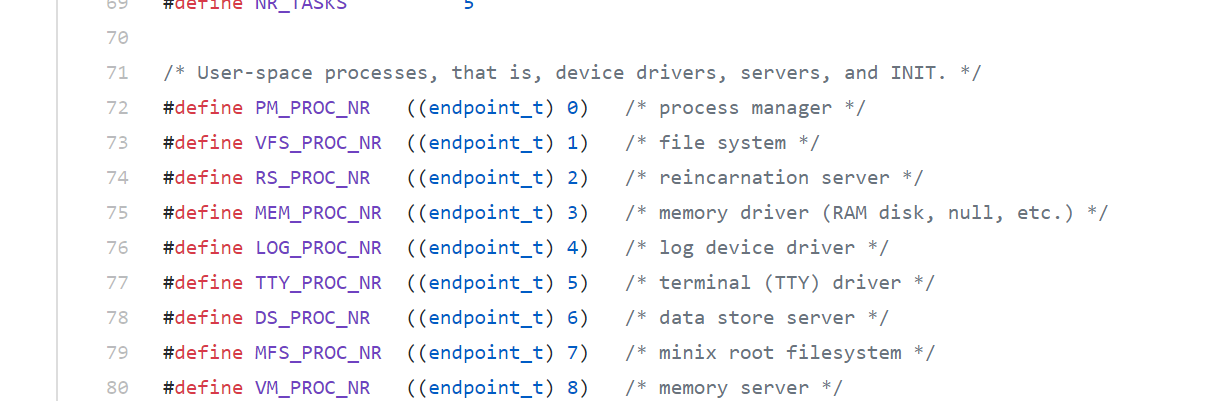
\includegraphics[scale=0.25]{fig/rc5_const}
\end{figure}
Problem of this design:
\begin{itemize}
	\item You need to keep track of the number for collision.
	\item These are handled by preprocessor.
	\item Accessible every where, assigning constants of \texttt{SPADE} to a variable of \texttt{FileType} doesn't make sense. 
\end{itemize}
\end{frame}

\begin{frame}{Critique on enumeration type}
\begin{itemize}
	\item Enumeration type in C++ is tightly connected to integer types. You probably need to constantly change them into integers / from integers. 
	\item Enumeration type lacks NULL/Invalid number. The compiler also doesn't keep track how many discrete value are there. 
	\item The process of reading an enumeration from user input usually involves a large switch. We need to keep retyping the name of the enumeration item. This is no better than a simple \texttt{const}.
	\item They are still accessible everywhere! You can access the enumeration item without specifying the category of the value.
	\item Take a look at C++ 11's newly (not very new after all) introduced \textit{Enumeration Class} for more detail. 
\end{itemize}
\end{frame}

\begin{frame}[fragile]{Buffer, flush and performance}
\textit{Buffering} have a potential problem. If your program crashed at some point, information in the buffer will be lost and thus not print out (for this reason \texttt{cerr} is not buffered). And there is an extra overhead of maintaining the consistence of the C++ style streamed IO with C style \texttt{printf}, \texttt{puts}... 

Why do we need such buffer? The reason is actually performance, flushing the buffer, or printing things onto the screen requires an interaction with the operating system, which is very expensive!

Buffer is an attempt the number of such interaction by trying to send as much text as possible out at once. Compare:

\begin{minted}{c++}
for (int i=0; i<10000; i++) cout << "Hello" << endl;
for (int i=0; i<10000; i++) cout << "Hello" << "\n";
\end{minted}
Generally the first one could be at least 3 times slower than the second one. This will be significant in the runtime of your program since your projects are often IO heavy (outputs a lot).
\end{frame}

\begin{frame}[fragile]{Tips on working with input stream}
\framesubtitle{Avoid parsing whenever possible!}
Specifically, avoid using \texttt{getline()} and \texttt{getch()} whenever possible. The C++ extractors has a very nice property: if you try to extract numbers or strings, the extractor automatically ignores blank characters. This means you only need to focus on the question of 
\begin{center}
	\textit{WHAT is the next thing I need?}
\end{center}

instead of thinking 
\begin{itemize}
	\item WHERE is the next thing I need?
	\item Is what I need on the next line?
	\item Is there a space or a tab before what I need?
	\item How do I get rid of that space / tab / newline?
\end{itemize}
\end{frame}

\begin{frame}[fragile]{Tips on working with input stream}
\framesubtitle{A VG101 Problem}
Recall the following VG101 problem (guess lots of you suffered...):
\begin{figure}
	\centering
	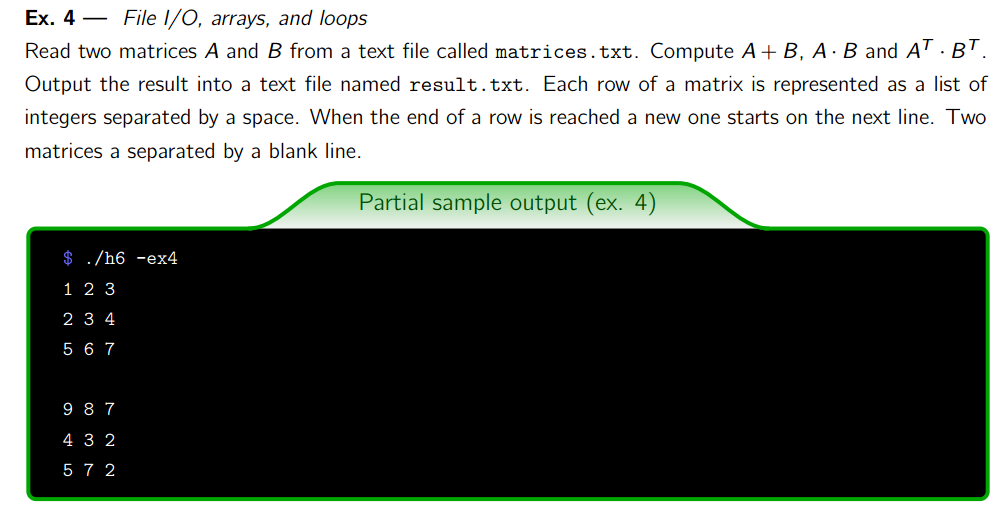
\includegraphics[scale=0.4]{fig/rc5_vg101}
\end{figure}
\end{frame}

\begin{frame}[fragile]{Tips on working with input stream}
\framesubtitle{The failed state}
If you try to extract invalid things from the stream, the stream enters a so called \textit{Failed State}. 

Two typical situation where a input stream will enter a fail state is when you try to extract things from an empty stream (all things in the stream has be extracted). Or you extracted the wrong type.

In general the second situation should be avoided. If you are not sure what next thing is, use a string to accept it. Transform the string into expected type later.

You can test whether a stream is in a valid state (very often if there is still thing remains in the stream) by simply \texttt{if(stream)}.

A very commonly used idiom to extract everything is:

\begin{minted}{c++}
int num; while(cin >> num) /* Do something here */;
\end{minted}

Please note that extractor operator returns an reference of the left hand stream.
\end{frame}

\begin{frame}[fragile]{Tips on working with file streams}
File streams are very much like \texttt{cin} or \texttt{cout}. Please note the difference of \texttt{ifstream} and \texttt{ofstream} and \texttt{fstream}. 

File streams can be opened on construction:
\begin{minted}{c++}
ifstream inputFileStream("input.txt");
\end{minted}
Above code opens \texttt{input.txt} with a \texttt{ifstream}. Please note if the file doesn't exist or failed to open, your \texttt{inputFileStream} will be in a failed state. Remember to check!

Although you can use \texttt{inputFileSteam.close()} to close the stream (and clear its buffer), but you don't actually need to. Remember the stack unwinding example we have before? Standard libraries' file stream are exactly such objects. Its deconstructor will take care of the closing and freeing the file.

\end{frame}

\begin{frame}[fragile]{Use \texttt{istringstream} as parser }
A \texttt{stringstream} can either act be an input stream, or an output stream. They are very different! 

\texttt{istringstream} needs to be ``attached" to a string. This can be down by either passing the string in on construction or use its \texttt{.str()} method. The stringstream, unlike \texttt{cin}, doesn't consume the string, instead it attach a ``pointer" to the string. Ideally:

\begin{minted}{text}
123 abc def Hello world  |  123 abc def Hello world
|<-sstream               |     |<-sstream 
\end{minted}

Right side is after extracting 123 through \texttt{sstream >> intVar;}

\texttt{istringstream} is especially useful in treating data acquired from \texttt{getline}. 

 \alert{If you need to use the same \texttt{istringstream} object for multiple strings, you need to clear it when changing string}. 
\end{frame}

\begin{frame}[fragile]{Use \texttt{ostringstream} as string builder}
From time to time we need to convert different type of data into a string. For example, information about a student is described by:
\begin{minted}{c++}
strcut Student {
    string name; int grade; Date birthday; double GPA;
};
\end{minted}
And you need to turn such stuctures into below format
\begin{minted}{c++}
%name, %grade grade, %YYYY-MM-DD, gpa = %gpa"
\end{minted}
You can setup an \texttt{ostringstream}. You simply push into the stream as if it is \texttt{cout}, finally you call \texttt{ostringstream.str()} to get the result. 
\begin{minted}{c++}
oss << name << "," << grade << " grade" << ... 
\end{minted}
The design of the stream makes it very efficient in dealing with large amount of text. For example you can use it to prepare data to send over the Internet.
\end{frame}

\subsection{Recurse Recursively}
\begin{frame}{Recursion is the art of abstraction}
A typical processes of designing a recursive function goes as follows:
\begin{itemize}
	\item Be very clear first about the abstraction of the function you needed to input.
	\item Specify a base case, a set of input where the answer is immediately known (or can be calculated in a few steps).
	\item Assume that your abstraction actually works for input ``simpler" than the current input (closer to the base case). Use this assumption to build your program.
\end{itemize}
You might find these steps surprisingly similar to a mathematical induction. That's true. They are similar and that's very useful.
\end{frame}

\begin{frame}[fragile]{Recursion is the art of abstraction}
\begin{minted}{c++}
// REQUIRES: list is not empty
// EFFECTS:  returns largest element in the list
int largest(list_t list) {
    int first = list_first(list);
    list_t rest = list_rest(list);
    if (list_isEmpty(rest)) return first;
    return max(first, largest(rest));
}
\end{minted}
\begin{itemize}
	\item The abstraction is specified in the header.
	\item The base base is where list contains just one element.
	\item In the last line, assume abstraction works in simpler case (hope you see why \texttt{rest} is ``simpler" than \texttt{list}). Thus \texttt{largest(rest)} returns the largest of the remaining list.
	\item The largest number can either be the largest of the remaining number, or the first number. 
\end{itemize}
\end{frame}

\begin{frame}[fragile]{Example: Quick sort algorithm}
A quick sort algorithm sorts a array in a quick way (I know that sound like bullshxx!). But list basic steps as following:
\begin{itemize}
	\item Select an element in the array. We simply use the first element. We call this element \texttt{pivot}
	\item We need to \textit{partition} the array. We need to move the elements less than the pivot to the left and elements larger than pivot to the right. Note we assume on the order of the elements left of the pivot (or elements on the right of the pivot).
\begin{minted}{text}
6 5 3 8 -1 7 3 9 11 -4   | 5 3 -1 3 -4 6 8 7 9 11
|<- pivot                |             |<- pivot
\end{minted}
	\item Call \texttt{QuickSort} on the both sides of the pivot.
\end{itemize}
The majority of the work lies in the partition step. 
\end{frame}

\begin{frame}{A usual Quick Sort}
\texttt{$-->$ code/rc5qsort/nonrec.cpp}
\inputminted{c++}{code/rc5qsort/nonrec.cpp}
\end{frame}

\begin{frame}[fragile]{Our Quick Sort}
Suppose we are using our list interface (in the project!). 
\begin{itemize}
	\item Suppose \texttt{QuickSort} is a function that takes in a list and returns a sorted list. Remember this is abstraction. Base case is when the list is empty.
\begin{minted}{c++}
list_t qSort(list_t lst); // Returns sorted lst 
\end{minted}

	\item Our computation goes as follows, we first acquire a the partion-left part and partition-right part. We call \texttt{qSort} on both parts and concatenate left, pivot and right part:
\begin{minted}{c++}
list_t sorted = cat(qSort(left), pivot, qSort(right)) 
\end{minted}
	\item The left part are simply numbers less than pivot, the right part are simply numbers greater than pivot.
\begin{minted}{c++}
list_t left = filterLess(lst, pivot);
list_t right = filterGreater(lst, pivot);
\end{minted}
	\item And we are done. Now we simply copy everything into one place.
\end{itemize}
\end{frame}

\begin{frame}[fragile]{Our Quick Sort}
And here is the famous (almost) one-line quick sort
\begin{minted}{c++}
list_t qSort(list_t lst) {
   if (isEmpty(lst)) return lst;
   int pivot = list_first(lst);
   return concatenate(
       qSort(filterLess(list, pivot)),
       pivot,
       qSort(filterGreater(list, pivot))
   );
}
\end{minted}
Now it just leaves us to implement the filter function and the concatenate function. But these two functions should be very easy. You have implemented the filter function in your project right? 
\end{frame}

\begin{frame}{Why not references and pointers?}
Think about it, why this seems much easier (clearer, hopefully you do feel that way)? 

In the traditional code, all functions works on the same array. We must manually control the process of copying, moving, etc. We are thinking in terms of \textit{operations}, detailed step to be performed.

But the the new code, we can now begin think of data. We stop focusing on the concrete steps, but simply
\begin{center}
	What should I do with the data? \\What is the expected input and the expected output?
\end{center} 
It is the computation we needed to focus. 

This is not easy. The immutability of the data and the fact that all functions are pure allows us to do such thing. Every function does calculation on its own and does not impact the outside world.
\end{frame}

\begin{frame}[fragile]{Bridging the old perspective}
Consider the following problem:

\vspace{0.1in}
\structure{Write a function \texttt{isMoreOdd} that takes a list $(a_0, a_1, a_2, ..., a_n)$ and returns $\Sigma_{i=0}^n i^2a_i$ (we call this an $s$-sum) Assuming the list is non empty.}
\vspace{0.1in}

An example as follows:

\begin{minted}{text}
a_i: 6  5  3  8  -1  7  3 
 i : 0  1  2  3  4   5  6
\end{minted}

We follow our usual steps. The abstraction is self-explanatory. The base case is also easy (a single element list). But the problem lies in the third step. 

It seems that knowing $s$-Sum for for the rest of the list doesn't help on the reducing the problem to a simpler point. 

It would still be most desirable to have some sort of ``accumulator", something that registers a partial sum, a piece of information that ``sums" up the elements before a certain point.
\end{frame}

\begin{frame}[fragile]{Accumulator passing style}
This is still possible. Such construct is so common that gets its own name. We call this \textit{Accumulator passing style} (APS). 

\begin{minted}{c++}
int helper(list_t remain, int index, int acc) {
    if (isEmpty(remain)) return acc;
    acc += index * index * list_first(remain);
    return helper(list_rest(remain), index + 1, acc);
}
list_t strangeSum(list_t list) { 
    return helper(list, 0, 0); 
}
\end{minted}

How does this work? 

The essential idea is to sum up the necessary information into two (could be more) accumulators. We essentially created a sort of running sum.
\end{frame}

\begin{frame}[fragile]{Accumulator passing style}
We then further note the abstraction of the helper function.

The function \texttt{helper} takes the index of the first element in the remainder list and a partial sum of the elements before, and returns the $s$-sum of the entire list.

In this way we transform our original problem of finding out \texttt{helper(list, 0, 0)}. On each recurse call, we extract the first element, and use it to update our accumulators, and passed that on to the next call. 

\begin{minted}{text}
helper([6  5  3  8  -1  7  3], 0, 0)
helper([5  3  8  -1  7  3], 1, 0)
helper([3  8  -1  7  3], 2, 5)
helper([8  -1  7  3], 3, 17)
helper([-1  7  3], 4, 89)
helper([7  3], 5, 73)
helper([3], 6, 248) = helper([], 7, 356) :=356
\end{minted}
\end{frame}

\begin{frame}{Remarks}
\begin{block}{Understand APS in a broad sense}
	APS is extremely useful. In many sense this technique is very similar to loops, which you might feel more comfortable to deal with. On the other hand an accumulator can be more than just an sum of numbers. It could be any information you need to keep track of (for example, if the number before forms an arithmetic sequence, and if they do, what is the increment). 
\end{block}

\begin{block}{Recursion and correctness}
	It's extremely difficult to write correct code! It would be nice if we can formally prove that our code is correct. Since the usual procedural code involves state, this proof can be very complex. 
	
	But if you express the idea using abstraction, proving correctness is very simple and forward. A good recursion construction is almost always correct, and you can prove it! Write once and be free of testing and bug. What a nice thing!
\end{block}
\end{frame}

	\section{RC Week 6}
\subsection{Program Arguments}
\begin{frame}{A syntax}
\end{frame}

\subsection{Engineering correctness: Testing}
\begin{frame}{Correctness through testing}

\end{frame}
\subsection{Engineering robustness: Exceptions}
\begin{frame}{Breaking the abstraction}

\end{frame}

	\section{RC Week 7}
\subsection{Program Arguments}
\begin{frame}[fragile]{Syntax}	
The following program 
\begin{minted}{c++}
int main(int argc, char* argv[]) {
    for (int i = 0; i < argc; i++)
        cout << "argv[i] = " << argv[i]; << endl;
}
\end{minted}
If executed with \texttt{../run/a.out Hello "123 23" 123 23}:
\begin{minted}{text}
argv[0] = ../run/a.out
argv[1] = Hello
argv[2] = 123 23
argv[3] = 123
argv[4] = 23
\end{minted}
The first argument is always the ``program name". Keep in mind the actual arguments start with index \texttt{1}. The system essentially breaks the calling command by spaces and put each segment into an array.
\end{frame}

\begin{frame}[fragile]{An example}
The following program checks if there are more than $n$ arguments that begins with \texttt{'!'}, $n$ is the first argument.
\begin{minted}{c++}
int main(int argc, char* argv[]) {
    if (argc < 2) return -1; // At least 2 arguments.
    int n = atoi(argv[1]); // Second argument
    for (int i = 2; i < argc; i++)
        // Strings starg with 3rd argument
        if (argv[i][0] == '!') n--;
    if (n <= 0) cout << "Yes!" << endl;
    else cout << "No!" << endl;
    return 0;
}
\end{minted}
\end{frame}

	\section{RC Week 8}

\subsection{Working with class invariants}	
\begin{frame}{Invariants of a datatype}
We now take a look at the implementation side. From a implementation point of view, what's the difference between a list of integers, and a set of integers? 
\begin{itemize}
	\item Both of them probably are represented using an array.
	\item Both of them might need to keep track of current number of elements. 
\end{itemize} 
The major difference lies in the fact that when inserting an element, integer set must check whether the element already exists. It is the assumptions on the member that makes them different.

\vspace{0.05in}
Integer set has one more assumption than integer list. Each number in the array must be unique. Every operation of an integer set must start with this assumption, might broke it in the middle, but ends up with it.

\vspace{0.05in}
We will use your \texttt{IntSet} example in class for our discussion.
\end{frame}

\begin{frame}{Example of invariants}
\begin{columns}
	\column[]{.5\textwidth}
	
	\vspace{-.3in}
	\inputminted[fontsize=\small]{c++}{code/rc8intset/intset.h}
	
	Invariants:
	
	1) Numbers are arranged in \texttt{elts} sequentially from index zero.

	2) Number of elements in array equals to the value of \texttt{numElts}.
	
	3) Numbers are unique.
	\column[]{.6\textwidth}
	
	\vspace{-.25in}
	Guideline is:
	\begin{itemize}
		\item Methods  assume inv.s on entry.
		\item (Public) Methods must preserve inv.s on the moment of exit.
		\item Nobody cares what happens in the middle!
	\end{itemize}
	This way we safely claim invariants are always preserved for an class instance from an external point of view. 
	
	Analyze the methods:
	\begin{itemize}
		\item \texttt{insert} might broke all three.
		\item \texttt{remove} might broke 1) and 2).
		\item \texttt{const} methods will not break anything! One more advantage!
	\end{itemize}
\end{columns}
\end{frame}

\begin{frame}{Example of invariants: Implementing methods}
\begin{columns}
	\column[]{.5\textwidth}
	
	\vspace{-.3in}
	
	\inputminted[fontsize=\small,xleftmargin=1em, linenos]{c++}{code/rc8intset/intset.cpp}
	
	\column[]{.6\textwidth}
	
	\vspace{-.25in}
	
	Analyze the methods:
	\begin{itemize}
		\item L.9 checks inv.3 for uniqueness.
		\item L.7 checks inv.2 for capacity. If violation of inv cannot be recovered from, depending on how serious situation is you can \texttt{throw} or fail-fast.
		\item L.9 uses inv.1. We insert at the end, temporarily breaks invariance.
		\item L.9 operator \texttt{++} restores inv.
		\item Inv.3 ensures \texttt{remove} works.
		\item L.15 restores inv.1. L.16 restores inv.2. A significant amount of code is dedicated to preserving invs.
	\end{itemize}
\end{columns}
\end{frame}


\begin{frame}{Remarks on invariants}
We would like to note the following things:
\begin{center}
	\structure{The centric problem in choosing an implementation\\ for an ADT, is choosing the invariants.}
\end{center}
There are multiple ways to write an implementation an \texttt{IntSet} of course. The major difference of them, is they need to keep different invariants, and thus have different performance. 

For example, you have already seen \texttt{IntSet} implemented using a sorted array. The one extra invariant you need to keep is that elements are sorted. Based on that extra invariant:
\begin{itemize}
	\item Queries are much quicker.
	\item Deletion and insertion are slower (by a constant factor).
\end{itemize}
In VE281 you will see (many) other ways of implementing this IntSet, for example using hash tables, or balance trees. It is always helpful to understand what the invariant for an implementation.
\end{frame}

\begin{frame}{Invariants and bad practices}
Thinking about invariants immediately gives us hints on what are seemingly good, some even sounds terrific, but are actually pretty bad ideas. We now take a look at some of them.

\begin{description}[Alice]
	\small
	\item[Alice] I'd like to add a public method to \texttt{IntSet}, let's say \texttt{find()}, which takes an element, found it in the set, and returns an reference to that element. 
	\item [Bob] Why do you want to do that?
	\item [Alice] Well my code needs to modify elements in the array, a lot. This would significantly accelerate the process.
	\item [Bob] ...
	\item [Alice] Oh, I get it, it's a pretty bad idea. OK I have another idea, I want to add a method, \texttt{data()}, which returns the pointer to array, since my code needs to iterate through the set. 
	\item [Bob] ...
	\item [Alice] What if I return pointer to const?
	\item [Bob] ...
	\item [Alice] Well, I give up. It's not as easy as I thought.
\end{description}
\end{frame}

\begin{frame}{Invariants and bad practices}
Well Alice does have her point. Her requirements are very real and the solutions does solutions could work, but remember the words from \textit{Donald Knuth}:
\begin{quotation}
	\structure{Premature optimization is the root of all evil}.
\end{quotation}
Never trade correctness for performance in designing phase. 
\begin{itemize}
	\small
	\item 1st and 2nd change Alice proposed have the problem that the client could change the content of the internal array, without notifying the instance. There is by no means the instance can guarantee the new value won't violate uniqueness invariance.
	\item Now Alice proposes the third one. The \texttt{const} key word could prevent the element from being modified. But it exposes the implementation to outside. Now the fact that elements are stored in a linear array becomes part of the abstraction, you can no longer change that. The problem is, iterating through a set seems to be an important feature, we DO need that. Well, the correct solution is using iterators, you will know them later in this course.
\end{itemize} 
\end{frame}

\begin{frame}{Invariants and bad practices}
Well Alice does have her point. Her requirements are very real and the solutions does solutions could work, but remember the words from \textit{Donald Knuth}:
\begin{quotation}
	\structure{Premature optimization is the root of all evil}.
\end{quotation}
Never trade correctness for performance in designing phase. 
\begin{itemize}
	\small
	\item 1st and 2nd change Alice proposed have the problem that the client could change the content of the internal array, without notifying the instance. There is by no means the instance can guarantee the new value won't violate uniqueness invariance.
	\item Now Alice proposes the third one. The \texttt{const} key word could prevent the element from being modified. But it exposes the implementation to outside. Now the fact that elements are stored in a linear array becomes part of the abstraction, you can no longer change that. The problem is, iterating through a set seems to be an important feature, we DO need that. Well, the correct solution is using iterators, you will know them later in this course.
\end{itemize} 
\end{frame}

\begin{frame}{Invariants and the constructor}
\alert{Invariants are there as long as the object is there.} The earliest moment the object is created, is when it is defined. Classes, are just structures, in terms of memory. Structures contains undefined values when created, so naturally does the classes. 

\vspace{0.03in}
Think about \texttt{IntSet}, when the object is created, chances are \texttt{numElts} contains non-zero value, while your set should be empty.

\vspace{0.03in}
We need a mechanism, a function, that is invoked whenever the an instance is created. This function is called, and called always, to initialize the object, or more strictly, to setup the invariance.

\vspace{0.03in}
Such special functions are \alert{constructors}, or \alert{ctors} for short. From this point on it's important to think the initialization, not as assigning special values to member variables, but as invoking the constructor to setup invariants (together with the initial state, e.g. initialize the \texttt{IntSet} with one default element in it for whatever reason).
\end{frame}

\begin{frame}[fragile]{Constructors: Syntax}

\begin{columns}
	\column[]{.5\textwidth}
	
	\vspace{-.3in}
	The construct for \texttt{IntSet}:
	\inputminted[]{c++}{code/rc8intset/intset_ctor.h}
	
	
	\column[]{.6\textwidth}
	
	\vspace{-.65in}
	
	\begin{itemize}
		\small
		\item Ctors have same name as class.
		\item Ctors don't return anything. 
		\item Usually \texttt{public}, but could be \texttt{private} for special need.
		\item A class could have more than one ctor, depending on what the initial state should be. We say the constructor is overloaded.
		\item Ctors could take initialization list.
		\item Ctor is the first function being called when the object is created. Unfortunately ``created" is not as simple as it sounds.
		\item A ctor that does not take argument is called \texttt{a default ctor}. Every class must always have a ctor. If you don't specify \alert{any ctor}, a ctor is synthesized for you (under some conditions).
	\end{itemize}
\end{columns}
\tiny{* We left out copy/move constructors on purpose. You will learn them later.}
\end{frame}

\begin{frame}[fragile]{Constructors: Explanations}
We need to break down the words from previous slide. We first look at the first four lines. The first three seems direct. For the fourth one:
\begin{minted}{c++}
IntSet set1; // set1 is init to an empty set;
IntSet set2(10); // set2 contains single elem 10
\end{minted}

\begin{minted}{c++}
int foo(const IntSet& s1, const IntSet& s2);
foo(IntSet(), IntSet(10)); // Anymous construction
\end{minted}

Further more, latest C++ standard guarantees the following:
\begin{minted}{c++}
IntSet setx = IntSet();    // Same as set1 
IntSet sety = IntSet(10);  // Same as set2
IntSet setz = 10;          // Same as set2
\end{minted}
This is non-trivial, for reasons you will see one or two weeks later. This is called \textit{guaranteed copy elision}. Now some food for thought: 

Why \texttt{set1} is not initialized as \texttt{IntSet set1();} for consistency?
\end{frame}

\begin{frame}[fragile]{Constructors: Explanations}
We now question: Is constructor really the first function being called when created? Well that depends on how you understand ``created"! One should argue the ctor IS part of object creation.

\vspace{0.1in}
In fact, there are 4 steps (roughly) in creating an class instance.
\begin{enumerate}
	\item Allocation of space, we (in general) don't have control over.
	\item Construction of the base class object.
	\item Construction of the members of current class.
	\item Calling the constructor.
\end{enumerate}
These 4 steps goes recursively. In fact the constructor is the last function being called. This is natural. 

When the constructor is called, we should be able to use all member variables and base class. So their invariants must have been setup in advance! This is the only way things makes sense.
\end{frame}

\begin{frame}[fragile]{Initializer list: Setup}
The \textit{initializer list}, the things after colon controls the second and third step. 

\begin{minted}{c++}
ClsName::ClsName() : base(..), m1(..), m2(..) {
    // Code for the constructor goes here
}
\end{minted}

%You might wonder, wait a minute, I have never write initializer list before, I don't even write a constructor!

To better illustrate our ideas, we make some changes to our original \texttt{IntSet}, specifically 2 changes:

\begin{itemize}
	\item We add a line of output to the ctors to indicate with constructor is being called.
	\item We make 2 more ``version" of our original \texttt{IntSet}, one \texttt{OddIntSet} and \texttt{EvenIntSet}. They only allow odd and even numbers, respectively.
\end{itemize}

We now propose a slightly faster \texttt{IntSet}. This \texttt{IntSet} is composed of an \texttt{OddIntSet} and \texttt{EvenIntSet}. It dispatches the operation on integers to those two sub-\texttt{IntSet}. 
%
%Well, if you don't provide any initializer list, the compiler calls the default constructor on every ctor, if a default ctor is available. If the default ctor is not available, a compile error is thrown.
\end{frame}

\begin{frame}[fragile]{Initializer list: Setup}
The \textit{initializer list}, the things after colon controls the second and third step. 

\begin{minted}{c++}
ClsName::ClsName() : base(..), m1(..), m2(..) {
    // Code for the constructor goes here
}
\end{minted}



To better illustrate our ideas, we make some changes to our original \texttt{IntSet}, specifically 2 changes:

\begin{itemize}
	\item We add a line of output to the ctors to indicate with constructor is being called.
	\item We make 2 more ``version" of our original \texttt{IntSet}, one \texttt{OddIntSet} and \texttt{EvenIntSet}. They only allow odd and even numbers, respectively.
\end{itemize}

We now propose a slightly faster \texttt{IntSet}. This \texttt{IntSet} is composed of an \texttt{OddIntSet} and \texttt{EvenIntSet}. It dispatches the operation on integers to those two sub-\texttt{IntSet}. 
%

\end{frame}

\begin{frame}[fragile]{Initializer list: Setup II}
\begin{columns}
	\column[]{.5\textwidth}
	
	\vspace{-.3in}
	Decl. of \texttt{OddIntSet}
	\inputminted[fontsize=\small]{c++}{code/rc8init/oddintset.h}
	
	\column[]{.5\textwidth}
	
	\vspace{-.3in}
	Partial implementation:
	\inputminted[fontsize=\small]{c++}{code/rc8init/oddintset.cpp}
\end{columns}

We omit the very similar version for \texttt{EvenIntSet}.
\end{frame}

\begin{frame}[fragile]{Initializer list: Setup III}
\begin{columns}
	\column[]{.5\textwidth}
	
	\vspace{-.2in}
	Declaration of \texttt{OddIntSet}
	\inputminted[fontsize=\small]{c++}{code/rc8init/fastintset.h}
	
	\column[]{.5\textwidth}
	
	\vspace{-.2in}
	Partial implementation:
	\inputminted[fontsize=\small]{c++}{code/rc8init/fastintset.cpp}
\end{columns}

\end{frame}

\begin{frame}[fragile]{Initializer list: Example}
We create a main function and instantiate an instance of \texttt{FastIntSet}. We observe the following ouput:
\begin{minted}{text}
OddIntSet dft ctor
EvenIntSet elt ctor
fIntSet ctor
\end{minted}
This implies an initialization order of \texttt{oddSet-evenSet-ctor}. This follows from our expectation. 

\vspace{0.1in}
A (not so important) remark we would like to make is
\begin{itemize}
	\item The order of initialization of the members is guaranteed by standard. It's NOT a UB!
	\item Contrary to intuition \textit{it is not specified by initializer list}, but by the order they appear in the declaration.
	\item Base objects are guaranteed to be initialized before members.
	\item We recommend you to specify the init-list in the same order as the declaration, for clearance.
\end{itemize}
\end{frame}

\begin{frame}[fragile]{Initializer list: Default initialization}
We now make a tiny change to the original setup. We change the ctor for \texttt{FastIntSet} to 
\begin{minted}{c++}
FastIntSet::FastIntSet() 
    : oddSet() {cout << "fIntSet ctor\n";}
\end{minted}

Oops, we forgot to specify initializer for \texttt{evenSet}.

\begin{minted}{text}
OddIntSet dft ctor
EvenIntSet dft ctor
fIntSet ctor
\end{minted}

\texttt{evenSet} is still initialized, no surprise, otherwise the invariant for \texttt{oddSet} would be broken. Members are default constructed, if they don't appear in the initializer list. We could even simply write 

\begin{minted}{c++}
FastIntSet::FastIntSet() {cout << "fIntSet ctor\n";}
\end{minted}

Which will produce the same result. Now what about members like \texttt{int}? Well, you can think of them as a class, whose default constructor does nothing at all!
\end{frame}

\begin{frame}[fragile]{Initializer list: Default initialization}
We can even leave out the constructor for \texttt{FastIntSet} entirely. In which case we would have the following output.

\begin{minted}{text}
OddIntSet dft ctor
EvenIntSet dft ctor
\end{minted}

Essentially the compiler would synthesize (create) and constructor for you, whose initializer list initializes everything using their default constructor.  

You might wonder, wait a minute, I have never write initializer list before, I don't even write a constructor before this lesson! That's how you ``get away" with writing constructors before!

Modern design principal is against leaving things unspoken. If you believe you only need a default constructor, you could do:

\begin{minted}{c++}
IntSet::InSet() = default; // In class decl.
\end{minted}

Next up we will look at something that is not taught in class, but problems you will meet in your own struggle with C++.
\end{frame}

\begin{frame}[fragile]{Initializer list: Default initialization}
We first change the ctor of \texttt{FastIntSet} to 
\begin{minted}{c++}
FastIntSet::FastIntSet() 
    : oddSet() {cout << "fIntSet ctor\n";}
\end{minted}

Then we \textbf{remove the default ctor} for \texttt{EvenIntSet}.

We compile the program. The question is what SHOULD happen?

\pause
\vspace{0.1in}
From a design point of view, if a class does not provide a default constructor, indicates the class is not (more likely should not be) default constructible, there is no way to setup a invariance without supplying an argument. Think about it, what should be the default skin color for an instance of a human class? None.

In this case, any reasonable design would require an compile error is thrown. This is exactly the case. They compiler will look for \texttt{evenIntSet::evenIntSet()} and reports a not-found error. \alert{Situation is similar if you leave out the entire ctor of \texttt{FastIntSet}.}
\end{frame}

\begin{frame}{Why initializing in initialization list is better?}
You are asked this question in the lecture slides but the question is left unanswered in the lecture slides.

\vspace{0.1in}
Frankly the questions really should be the other way around: on what grounds do initialization in the code is better? I can think of the following reasons you should prefer (in some cases you have to use) initialization list:
\begin{itemize}
	\item Performance. This will be discussed later on. In some cases the performance could be significant.
	\item Exception safety. We will discuss this when we you learn the rule of big three (five, actually).
	\item A member that don't have a default constructor must be initialized in the initialization list.
	\item \texttt{const} members and references can only be initialized in the initialization list.
	\item Semantic reasons.
\end{itemize} 
\end{frame}

\begin{frame}[fragile]{Comments on the performance argument}
A final comment on the performance argument. Suppose we write 
\begin{minted}{c++}
FastIntSet::FastIntSet() {
  cout << "fIntSet ctor\n";
  oddSet = OddIntSet(); evenSet = eventSet(10);
}
\end{minted}
You will observer 5 lines of output:
\begin{minted}[fontsize=\small]{text}
OddIntSet dft ctor // EvenIntSet dft ctor //
fIntSet ctor // OddIntSet dft ctor // EvenIntSet elt ctor //
\end{minted}
Things that actually happened (with significant cost) are :
\begin{itemize}
	\item Your member variables are first default constructed.
	\item Calls your constructor.
	\item You create 2 temporal objects, by default construction.
	\item You invoke an assignment operator and uses your temporal object to overwrite the member variables. 
\end{itemize}

\end{frame}

\end{document}